% =====================================================================
%  Almost-idempotent positive maps and approximate Jordan algebras
%  Self-contained report. Main file: structure only; content in sections/.
%  Build:  make   (or: latexmk -pdf main.tex)
%
%  PROVENANCE POLICY (see PROVENANCE.md):
%   - Every Definition and Theorem carries a `% PROV:` comment naming the
%     ground-truth source file and the source locus it is matched to.
%   - PROVENANCE.md is the audit ledger (source path, SHA256, source locus).
%   - No claim without a provenance entry. No jargon without a definition.
% =====================================================================
\documentclass[11pt]{article}

\usepackage[T1]{fontenc}
\usepackage[utf8]{inputenc}
\usepackage{amsmath,amssymb,amsthm,mathtools}
\usepackage{booktabs}
\usepackage{graphicx}
\usepackage{xcolor}
\usepackage[margin=1in]{geometry}
\usepackage{enumitem}
\usepackage[colorlinks=true,linkcolor=blue,citecolor=blue,urlcolor=blue]{hyperref}
\usepackage{cleveref}

% ---- theorem environments ----
\theoremstyle{plain}
\newtheorem{theorem}{Theorem}[section]
\newtheorem{lemma}[theorem]{Lemma}
\newtheorem{proposition}[theorem]{Proposition}
\newtheorem{corollary}[theorem]{Corollary}
\newtheorem{openproblem}[theorem]{Open Problem}
\theoremstyle{definition}
\newtheorem{definition}[theorem]{Definition}
\newtheorem{remark}[theorem]{Remark}
\newtheorem{example}[theorem]{Example}
\crefname{openproblem}{open problem}{open problems}
\Crefname{openproblem}{Open Problem}{Open Problems}

% ---- notation macros (kept minimal and explicit) ----
% Symbol macros are wrapped in \ensuremath so they are mode-agnostic
% (usable in both text and math without "Missing $" errors).
\newcommand{\R}{\ensuremath{\mathbb{R}}}
\newcommand{\C}{\ensuremath{\mathbb{C}}}
\newcommand{\HH}{\ensuremath{\mathcal{H}}}            % Hilbert space
\newcommand{\Bsa}{\ensuremath{B(\HH)_{\mathrm{sa}}}}  % self-adjoint operators
\newcommand{\jp}{\ensuremath{\circ}}                  % Jordan product
\newcommand{\norm}[1]{\ensuremath{\lVert #1 \rVert}}
\newcommand{\Id}{\ensuremath{\mathbf{1}}}             % unit element / identity operator
\newcommand{\Tr}{\ensuremath{\operatorname{Tr}}}
\newcommand{\Img}{\ensuremath{\operatorname{Im}}}
\newcommand{\Ker}{\ensuremath{\operatorname{Ker}}}
\newcommand{\Aut}{\ensuremath{\operatorname{Aut}}}
\newcommand{\sgn}{\ensuremath{\operatorname{sgn}}}
\newcommand{\Phimap}{\ensuremath{\Phi}}
\newcommand{\eps}{\ensuremath{\varepsilon}}
\newcommand{\status}[1]{\textnormal{\textsc{#1}}}
% Provenance marker (renders nothing; the audit lives in PROVENANCE.md, keyed by label)
\newcommand{\prov}[1]{}

% ---- af-validation links ------------------------------------------------------
% A result tagged \afbadge{<id>} is machine-checked in the adversarial proof
% framework; the badge links to its af workspace proofs/<id>/ on GitHub (the
% registry id == the proofs/ directory name). \aflink renders custom link text;
% \afyes is the bare green tick used in the status ledger column.
\definecolor{afgreen}{rgb}{0,0.45,0}
\newcommand{\afbadge}[1]{\,{\footnotesize\textsf{\textcolor{afgreen}{$\checkmark$\,\href{https://github.com/tobiasosborne/almost-idempotent-positive-maps/tree/main/proofs/#1}{af-validated}}}}}
\newcommand{\aflink}[2]{\href{https://github.com/tobiasosborne/almost-idempotent-positive-maps/tree/main/proofs/#1}{\textcolor{afgreen}{#2}}}
\newcommand{\afyes}{\textcolor{afgreen}{$\checkmark$}}

\title{Almost-idempotent positive maps\\ and approximate Jordan algebras}
\author{Agent A \and Agent B\\[2pt]\small (collaborative working report)}
\date{\today}

\begin{document}
\maketitle

\begin{abstract}
Kitaev showed that a quantum channel which is almost idempotent --- a unital
completely positive map $\Phi$ on the operators of a finite-dimensional Hilbert
space with $\norm{\Phi^2-\Phi}_{\mathrm{cb}}\le\eta$ --- carries, on its
near-fixed points, the structure of an approximate $C^*$-algebra, and that every
finite-dimensional approximate $C^*$-algebra is close to a genuine one. We study
the same question when $\Phi$ is only assumed \emph{positive}, not completely
positive. We show that the correct invariant is then a \emph{Jordan} algebra
rather than an associative one, for a precise structural reason: a positive
unital map need not satisfy the Schwarz inequality $\Phi(x)^*\Phi(x)\le
\Phi(x^*x)$, but it always satisfies Kadison's inequality $\Phi(x)^2\le\Phi(x^2)$
for self-adjoint $x$, and the latter involves exactly the data of a Jordan
algebra.

Our main complete result is a \emph{bridge theorem}: for any unital positive
$\Phi$ with $\norm{\Phi^2-\Phi}\le\eta$, the near-fixed-point space
$A=\Img P$ of the spectral idempotent $P=\theta(2\Phi-\Id)$, equipped with the
product $a\bullet b=P(a\jp b)$, satisfies the axioms of a Jordan algebra up to
an error $O(\sqrt\eta)$, with constants independent of dimension. The proof uses
no dilation and no complete positivity; the key fact is that the ``square holes''
$P(a^2)-a^2$ are almost-positive null elements, so that quadratic error terms are
$O(\eta)$ while the exact Jordan identity of the ambient algebra cancels the
leading term.

We then carry the programme as far as it currently goes and report honestly on
what is proved, conditional, or open. \emph{(i)} We reduce \emph{exact}
factorization by unital positive maps to a single stability question
--- that a near-positive idempotent is $O(\sqrt\eta)$-close to a genuine positive
one --- proving the factorization conditional on it and showing that no
generic positivity-rounding can replace it. \emph{(ii)} In the commutative case
this becomes a stability problem for almost-idempotent stochastic matrices; we
record the sharp square-root exponent, several proved special cases, and an exact
commutative factorization theorem, leaving one geometric lemma open.
\emph{(iii)} For the abstract structure theorem --- every finite-dimensional
approximate Jordan algebra is close to a genuine one --- we present a
dimension-free splitting of the Jordan cohomology coboundary for exact cocycles
on every finite-dimensional JB-algebra (the exact-adjoint benchmark), isolating
the approximate-cocycle and positivity gaps that remain. \emph{(iv)} We analyse
the exponent ($1/2$ in general; $1$ for completely positive maps, and
conjecturally for decomposable maps, conditional on a dilation-compatibility
hypothesis that we make precise). The report is a consensus document of two
collaborating authors; every statement is tagged as a definition, a cited fact,
a proved result, a conditional result, or an open target.

\end{abstract}

\tableofcontents
\bigskip

\section{Introduction}\label{sec:intro}

\paragraph{The question.}
A physical system sometimes hides a smaller logical system inside it: the
logical observables are encoded in the physical ones, and a recovery operation
returns the system to the encoded subspace. Mathematically, such a recovery is a
quantum channel $T$ that is idempotent, $T^2=T$. Kitaev~\cite{Kitaev2024} studied
the realistic case where the recovery is only \emph{approximately} idempotent,
and asked what algebraic structure the encoded observables carry. He worked with
the dual map $\Phi$ of the channel, a unital completely positive map on the
algebra $B(\HH)$ of operators on a finite-dimensional Hilbert space, and measured
non-idempotence by $\norm{\Phi^2-\Phi}_{\mathrm{cb}}\le\eta$. His answer: the
near-fixed points of $\Phi$ form an \emph{approximate $C^*$-algebra}, and every
finite-dimensional approximate $C^*$-algebra is, with universal (dimension-free)
constants, close to a genuine $C^*$-algebra.

\paragraph{This report.}
We ask the same question for maps that are only \emph{positive}, not completely
positive. This is the natural setting whenever one cares about distinguishability
of states rather than full quantum operations, and it is the setting of
van~Luijk and Wilming~\cite{vanLuijkWilming2026}, who show that for positive
trace-preserving maps the relevant invariant is a \emph{Jordan} algebra. The
present report does three things, in order of completeness:
\begin{enumerate}[leftmargin=*]
  \item It records the consensus \emph{definitions} (positive map, Jordan
    product, JB-algebra, order-unit space, approximate Jordan algebra). Standard
    background definitions are matched against local source copies; project
    definitions such as the $\eps$-JB notion are marked \status{(consensus)} and
    tied to internal proof files in \texttt{PROVENANCE.md}.
  \item It proves the \emph{bridge theorem} (\Cref{sec:bridge}): from a unital
    positive almost-idempotent $\Phi$ one obtains, with no use of dilations or
    complete positivity, a space that satisfies the Jordan-algebra axioms up to
    $O(\sqrt\eta)$. This is the positive-map analogue of the first half of
    Kitaev's construction, and it is complete.
  \item It states the \emph{structure-theory programme} (\Cref{sec:programme})
    --- the analogue of the second half of Kitaev's theorem --- and reports
    precisely what is established and what is still open
    (\Cref{sec:discussion}).
\end{enumerate}

\paragraph{Why Jordan, and not associative.}
The reason positivity forces a Jordan, rather than associative, structure can be
stated in one line. Kitaev's verification of the $C^*$-norm axiom rests on the
Schwarz inequality $\Phi(x)^*\Phi(x)\le\Phi(x^*x)$, which holds for $2$-positive
(in particular completely positive) maps. A merely positive unital map need not
satisfy it; what it does satisfy is Kadison's inequality
$\Phi(x)^2\le\Phi(x^2)$ for self-adjoint $x$~\cite{Kadison1952}. The latter
involves only self-adjoint elements and squares --- exactly the data on which a
Jordan algebra is built. Replacing the associative product $xy$ by the symmetric
product $x\jp y=\tfrac12(xy+yx)$ throughout is therefore not a convenience but a
necessity, and the entire theory reorganises around it.

\paragraph{Conventions and status flags.}
All Hilbert spaces are finite-dimensional and complex. We write $B(\HH)$ for the
operators on $\HH$ and $\Bsa$ for the self-adjoint ones. Statements carry a
status: \status{(proved)} for results with a complete proof in this report;
\status{(cited)} for results transcribed verbatim from a named source;
\status{(consensus)} for definitions and conventions adopted by agreement
between the authors (a definition is never ``proved''); and \status{(open)} for
targets of the programme not yet established. Constants denoted $C$ are universal and never depend on
$\dim\HH$ unless explicitly stated.

\section{Preliminaries}\label{sec:prelim}

This section fixes the analytic setting. Everything is finite-dimensional; the
only norm is the operator norm, and the only positivity used is positivity of
maps (never complete positivity).

% PROV: Idel2013 md:333 -- self-adjoint part and positive semidefinite order for matrices. HancheOlsenStormer1984 joa-m.md:374 -- states on an order-unit space are positive functionals rho with rho(e)=1.
\begin{definition}[Operators, self-adjoint part, states]\label{def:operators}
\status{(cited)}
Let $\HH$ be a finite-dimensional complex Hilbert space and $B(\HH)$ the algebra
of linear operators on $\HH$, with the operator norm
$\norm{x}=\sup_{\norm{\xi}\le 1}\norm{x\xi}$. The \emph{self-adjoint part} is
$\Bsa=\{x\in B(\HH):x=x^*\}$, a real vector space. For $a\in\Bsa$ we write
$a\ge 0$ if every eigenvalue of $a$ is nonnegative; this induces the partial
order $a\ge b\iff a-b\ge 0$, with unit $\Id$ the identity operator. A
\emph{state} is a linear functional $\omega:B(\HH)\to\C$ that is positive
($\omega(a)\ge 0$ for $a\ge 0$) and unital ($\omega(\Id)=1$).
\end{definition}

% PROV: Idel2013 md:347-348 -- "positive if for all A>=0, T(A)>=0"; "unital if T(1)=1". The order-unit norm contraction is proved inline from the order interval.
\begin{definition}[Positive, unital, and positive unital maps]\label{def:positive-map}
\status{(cited)}
A linear map $\Phimap:B(\HH)\to B(\HH)$ is \emph{positive} if $\Phimap(a)\ge 0$
whenever $a\ge 0$; a positive map is automatically self-adjointness-preserving,
$\Phimap(a^*)=\Phimap(a)^*$, so it restricts to a real-linear map
$\Phimap:\Bsa\to\Bsa$. It is \emph{unital} if $\Phimap(\Id)=\Id$. A
\emph{positive unital map} is a contraction on the self-adjoint part: for
$a\in\Bsa$ one has $-\norm a\,\Id\le a\le\norm a\,\Id$, hence
$-\norm a\,\Id\le\Phimap(a)\le\norm a\,\Id$ by positivity and unitality, so
$\norm{\Phimap(a)}\le\norm a$; with $\Phimap(\Id)=\Id$ this gives
$\norm{\Phimap}=1$ on $\Bsa$.
\end{definition}

The order structure of $\Bsa$ is what survives when the associative product is
dropped; it is captured abstractly by the notion of an order-unit space.

% PROV: HancheOlsenStormer1984 joa-m.md:366-372 (1.2.1) -- order unit, Archimedean, order norm
\begin{definition}[Order-unit space and order-unit norm]\label{def:order-unit}
\status{(cited)}
A real vector space $A$ with a proper convex cone $A^{+}$ (giving
$a\ge b\iff a-b\in A^{+}$) and a distinguished element $e\in A^{+}$ is an
\emph{order-unit space} if (i) $e$ is an \emph{order unit}: for each $a\in A$
there is $\lambda>0$ with $-\lambda e\le a\le\lambda e$, and (ii) $A$ is
\emph{Archimedean}: $na\le e$ for all $n\in\mathbb N$ implies $a\le 0$. The
\emph{order-unit norm} is
\[
  \norm a=\inf\{t>0:\ -t\,e\le a\le t\,e\}.
\]
With $e=\Id$ and cone $A^{+}=\{a\in\Bsa:a\ge 0\}$, the self-adjoint part $\Bsa$
is an order-unit space, and its order-unit norm coincides with the operator norm.
\end{definition}

\begin{remark}\label{rem:order-unit-justification}
\status{(proved)}
That $\Bsa$ is an order-unit space is immediate from
\Cref{def:order-unit}: for self-adjoint $a$, the spectral bound
$-\norm a\,\Id\le a\le\norm a\,\Id$ shows $\Id$ is an order unit and that the
order-unit norm equals the spectral-radius (operator) norm; the Archimedean
property holds because $\Bsa$ is finite-dimensional. In the channel setting of
this report the order-unit structure of the relevant subspace is inherited
\emph{exactly} from $\Bsa$; only the product will be approximate.
\end{remark}

The single positivity inequality available for merely positive unital maps is
Kadison's, with its symmetrized strengthening due to St{\o}rmer.

% PROV: Kadison1952 -- Kadison's inequality Phi(a)^2 <= Phi(a^2) for self-adjoint a, unital positive Phi
% (also stated in report intro 01-introduction.tex; cited there to Kadison1952)
\begin{proposition}[Kadison and Jordan--Schwarz inequalities]\label{prop:kadison-js}
\status{(cited)}
Let $\Phimap:B(\HH)\to B(\HH)$ be a positive unital map.
\begin{enumerate}[label=(\roman*),leftmargin=*]
  \item \emph{(Kadison~\cite{Kadison1952})} For every self-adjoint $a\in\Bsa$,
        \[
          \Phimap(a)^2\ \le\ \Phimap(a^2).
        \]
  \item \emph{(Jordan--Schwarz, St{\o}rmer~\cite{Stormer1965,vanLuijkWilming2026})}
        For every $a\in B(\HH)$, writing $\jp$ for the Jordan product
        $x\jp y=\tfrac12(xy+yx)$,
        \[
          \Phimap(a^*)\jp\Phimap(a)\ \le\ \Phimap(a^*\jp a).
        \]
\end{enumerate}
Part (i) is the case $a=a^*$ of part (ii). A merely positive unital map need not
satisfy the Schwarz inequality $\Phimap(a)^*\Phimap(a)\le\Phimap(a^*a)$, which
requires $2$-positivity.
\end{proposition}

% PROV: ORIGINAL agent-a-findings:20,191 -- cb-norm/complete positivity used only in tensor extension; no cb-norm here
\begin{remark}[Operator norm in place of the cb-norm]\label{rem:cb-norm}
\status{(proved)} \emph{(framing; original to this report)}
Kitaev~\cite{Kitaev2024} measures non-idempotence in the completely bounded
norm, $\norm{\Phimap^2-\Phimap}_{\mathrm{cb}}\le\eta$, which presupposes that the
relevant maps are completely bounded. We instead use the operator norm of the
map on $\Bsa$, $\norm{\Phimap^2-\Phimap}\le\eta$. The reason is structural:
mere positivity is not stable under matrix amplification:
$\mathrm{id}_n\otimes\Phimap$ need not be positive. In finite dimension every
linear map is bounded (and completely bounded once an operator-space structure
is fixed), so the obstruction is not existence of a cb-norm; it is that the
cb/tensor norm is not the order-norm control supplied by positivity alone.
The cb-norm and complete positivity enter Kitaev's argument only through the
dilation/tensor machinery (Stinespring, Choi); the operator-norm formulation
keeps every estimate intrinsic to $\Bsa$ and dilation-free, at the cost of the
weaker exponent recorded in the bridge theorem (\Cref{sec:bridge}). Throughout,
the spectral idempotent is denoted $P$ and the projected Jordan product is
written $a\bullet b:=P(a\jp b)$.

\smallskip\noindent\textbf{Agent B review correction.}
The earlier draft said that a positive map need not be completely bounded. In
the finite-dimensional setting of this report that sentence is false; the
correct issue is failure of positivity under amplification.
\end{remark}

\section{Jordan algebras and JB-algebras}\label{sec:jordan}

This section fixes the algebraic vocabulary used throughout the report. Every
object here is standard; we follow the axioms in Hanche-Olsen and
St{\o}rmer~\cite{HancheOlsenStormer1984} so that later approximate versions
(\Cref{sec:epsjb}) can be read as quantitative relaxations of these exact
identities. We work over a field of characteristic not $2$; for the analytic
results the scalars are real, as indicated.

\subsection{Jordan algebras}

The Jordan product symmetrises an associative product: for operators on a Hilbert
space, $a\jp b=\tfrac12(ab+ba)$ is self-adjoint whenever $a$ and $b$ are, so it
keeps us inside $\Bsa$ where the associative product $ab$ does not. Abstracting
the two identities that this symmetrised product satisfies gives the notion of a
Jordan algebra.

% PROV: HancheOlsenStormer1984 line 812 (eq 2.17) and lines 963-967 (item 2.4.1, eqs 2.29-2.30) -- Jordan product and the two defining axioms.
\begin{definition}[Jordan algebra]\label{def:jordan-algebra}
\status{(cited)}
For elements $a,b$ of an associative algebra, the \emph{Jordan product} is
\begin{equation}\label{eq:jordan-product}
  a \jp b = \tfrac12(ab+ba).
\end{equation}
An algebra $A$ with a product written $(a,b)\mapsto a\jp b$ is called a
\emph{Jordan algebra} if the following two identities hold for all $a,b\in A$:
\begin{align}
  a \jp b &= b \jp a, \label{eq:jordan-comm}\\
  a \jp (b \jp a^2) &= (a \jp b) \jp a^2. \label{eq:jordan-identity}
\end{align}
Identity~\eqref{eq:jordan-comm} states that $A$ is commutative;
\eqref{eq:jordan-identity} is the \emph{Jordan identity}. Here $a^2 := a\jp a$.
\end{definition}

% PROV: HancheOlsenStormer1984 line 812 and lines 965-967; notation harmonised to \jp.

\begin{remark}[Form of the Jordan identity]\label{rem:jordan-identity-form}
\status{(cited)}
The Jordan identity~\eqref{eq:jordan-identity}, written
$a\jp(b\jp a^2)=(a\jp b)\jp a^2$ in~\cite{HancheOlsenStormer1984}, is the same as
the symmetric-looking form
\[
  \bigl((a\jp a)\jp b\bigr)\jp a \;=\; (a\jp a)\jp(b\jp a),
\]
obtained by writing $a^2=a\jp a$ and applying
commutativity~\eqref{eq:jordan-comm} to each product. We use whichever form is
more convenient; they are equivalent in any commutative algebra.
\end{remark}

A Jordan algebra need not be associative. Its one indispensable substitute for
associativity is that any single element, together with its powers, generates an
associative subalgebra. This is what makes a functional calculus possible later.

% PROV: HancheOlsenStormer1984 lines 1013-1025 (items 2.4.4-2.4.5) -- power-associativity: powers defined inductively and the subalgebra on one element is associative.
\begin{proposition}[Power-associativity]\label{prop:power-associative}
\status{(cited)}
Let $A$ be a Jordan algebra and $a\in A$. Define powers inductively by $a^1=a$
and $a^{n+1}=a\jp a^n$ (and $a^0=\Id$ if $A$ is unital). Then the subalgebra
generated by $a$ is associative; equivalently, for all natural numbers $m,n$,
\begin{equation}\label{eq:power-assoc}
  a^{m+n} = a^m \jp a^n .
\end{equation}
Consequently every power $a^n$ is unambiguously defined.
\end{proposition}

% PROV: HancheOlsenStormer1984 lines 1013-1017; notation harmonised to \jp.

\subsection{JB-algebras}

To do analysis one adds a complete norm compatible with the product. The two
extra norm conditions below are the Jordan analogue of the $C^*$-identity: the
first fixes the norm of a square, the second forces sums of squares to dominate
their summands and is what makes the order structure (positivity = being a
square) well-behaved.

% PROV: HancheOlsenStormer1984 lines 2308-2316 (items 3.1.3-3.1.4) -- Jordan Banach algebra and the two JB-algebra norm conditions.
\begin{definition}[JB-algebra]\label{def:jb-algebra}
\status{(cited)}
A \emph{Jordan Banach algebra} is a real Jordan algebra $A$ equipped with a
complete norm satisfying
\begin{equation}\label{eq:submultiplicative}
  \norm{a \jp b} \le \norm{a}\,\norm{b}, \qquad a,b\in A.
\end{equation}
A \emph{JB-algebra} is a Jordan Banach algebra $A$ whose norm satisfies, in
addition, the following two conditions for all $a,b\in A$:
\begin{align}
  \norm{a^2} &= \norm{a}^2, \label{eq:jb-square}\\
  \norm{a^2} &\le \norm{a^2 + b^2}. \label{eq:jb-sum-of-squares}
\end{align}
If $A$ is unital with unit $\Id$, then~\eqref{eq:jb-square} gives $\norm{\Id}=1$.
\end{definition}

% PROV: HancheOlsenStormer1984 lines 2308-2316; source drops the hyphen in "JB-algebra" by a typesetting error noted at line 13; we restore it.

The motivating example is concrete: for a complex Hilbert space $\HH$, the
self-adjoint operators $\Bsa$ form a JB-algebra under~\eqref{eq:jordan-product}
and the operator norm. A norm-closed Jordan subalgebra of some $\Bsa$ is called a
\emph{JC-algebra}~\cite[3.1.2]{HancheOlsenStormer1984}, and every JC-algebra is a
JB-algebra. The content of the finite-dimensional theory is that, with one
exception, the converse also holds.

\subsection{Finite-dimensional classification}

In finite dimensions the JB-algebras are exactly the classical objects of
Jordan, von Neumann and Wigner~\cite{JordanVonNeumannWigner1934}: a real Jordan
algebra $A$ is called \emph{formally real} (or Euclidean) if
$\sum_{i=1}^n a_i^2 = 0$ in $A$ forces $a_1=\dots=a_n=0$. A finite-dimensional
unital formally real Jordan algebra is a JB-algebra in its order
norm~\cite[3.1.7]{HancheOlsenStormer1984}, and conversely every JB-algebra is
formally real~\cite[3.3.8]{HancheOlsenStormer1984}; so in finite dimensions the
two classes coincide. Their simple pieces are completely classified.

% PROV: HancheOlsenStormer1984 line 2254 (Theorem 2.9.6) together with line 2264 (2.9.7) and Theorem 2.9.8 (line 2270) -- classification of finite-dimensional simple formally real Jordan algebras; attributed to Jordan-von Neumann-Wigner [69] at line 2293.
\begin{theorem}[Jordan--von Neumann--Wigner classification]\label{thm:jnw-classification}
\status{(cited)}
Every finite-dimensional, formally real, unital Jordan algebra is a direct sum of
simple ones. Each simple summand is isomorphic to exactly one of
\begin{itemize}
  \item the one-dimensional algebra $\R$;
  \item a \emph{spin factor} $\R\Id\oplus H$, where $H$ is a real inner-product
    space of dimension $\ge 2$ (the case of two minimal projections summing
    to~$\Id$);
  \item a Hermitian matrix algebra $H_n(\R)$, $H_n(\C)$, or $H_n(\mathbb{H})$
    with $n\ge 3$, where $\mathbb{H}$ denotes the quaternions; or
  \item the \emph{Albert algebra} $H_3(\mathbb{O})$ of $3\times 3$ Hermitian
    matrices over the octonions $\mathbb{O}$.
\end{itemize}
Of these, only $H_3(\mathbb{O})$ is \emph{exceptional}: it is not isomorphic to a
Jordan subalgebra of self-adjoint operators on any Hilbert space; all the others
are JC-algebras.
\end{theorem}

\smallskip\noindent\textbf{Agent B review correction.}
The one-dimensional summand $\R$ is included explicitly; it is the $n=1$ case in
Hanche-Olsen--St{\o}rmer Theorem 2.9.6 and is not covered by the listed spin
factors.

% PROV: HancheOlsenStormer1984 line 2254 (2.9.6), line 2264 (2.9.7), line 1856 (Corollary 2.8.5), and line 2306; attribution at line 2293; original source JordanVonNeumannWigner1934.

\begin{remark}[Status of the exceptional algebra]\label{rem:exceptional}
\status{(cited)}
The exceptionality of $H_3(\mathbb{O})$ traces back to the non-associativity of
the octonions~\cite[2.8.5]{HancheOlsenStormer1984}. It is the only obstruction to
representing a finite-dimensional formally real Jordan algebra by self-adjoint
operators, and it is the reason the structure theory of \Cref{sec:programme} must
allow for a Jordan, rather than associative, limit object.
\end{remark}

\section{The spectral idempotent}\label{sec:spectral}

Throughout this section $\Phimap\colon\Bsa\to\Bsa$ is a fixed unital positive
linear map that is \emph{almost idempotent}: there is a parameter
$\eta\in[0,\tfrac14)$ with
\begin{equation}\label{eq:eta-hypothesis}
  \norm{\Phimap^2-\Phimap}\le\eta,
\end{equation}
where $\norm{\cdot}$ on the left is the operator norm of a linear map on
$\Bsa$ (the order-unit norm $\norm{x}=\inf\{t>0:-t\Id\le x\le t\Id\}$ being
used on $\Bsa$ itself). The goal is to replace $\Phimap$ by an honest
idempotent $P$ that is close to $\Phimap$ and inherits its order properties up
to an error of size $\eta$. The construction is Kitaev's; we record the
elementary bounds we need with explicit dependence on $\eta$.

We work inside the Banach algebra $\mathrm{End}(\Bsa)$ of bounded linear
operators on $\Bsa$, whose unit we also denote $\Id$. Since $\Phimap$ is
unital positive it is a contraction for the order-unit norm, so
$\norm{\Phimap}=1$.

% PROV: Kitaev2024 approximate_algebras.tex:2171-2182 (eq tilde_Phi) -- construction P=theta(2Phi-1)=(1/2)(1+(2Phi-1)(1-4(Phi-Phi^2))^{-1/2}); properties P^2=P, ||P-Phi||<=O(eta), P(1)=1, P(X^dag)=P(X)^dag in the complex setting. This report restricts to B_sa, where the relevant preservation statement is real self-adjointness preservation. Also Prop prop_P (lines 524-533) and abs_sgn (line 515).
\begin{definition}[Spectral idempotent, \status{(cited)}]\label{def:spectral-idempotent}
Set $S=2\Phimap-\Id\in\mathrm{End}(\Bsa)$. Define
\begin{equation}\label{eq:R-binomial}
  R=(S^2)^{-1/2}
\end{equation}
by the binomial series for $(\Id-(\Id-S^2))^{-1/2}$, set
$\sgn(S)=SR$, and put
\begin{equation}\label{eq:P-def}
  P=\theta(2\Phimap-\Id)=\tfrac12\bigl(\Id+\sgn(S)\bigr)
   =\tfrac12\Bigl(\Id+(2\Phimap-\Id)\bigl(\Id-4(\Phimap-\Phimap^2)\bigr)^{-1/2}\Bigr).
\end{equation}
This is the spectral idempotent of $\Phimap$ for the spectral cluster near
$1$ \cite[Eq.~(tilde\_$\Phimap$), Prop.~P]{Kitaev2024}.
\end{definition}

The series defining $R$ converges because $S^2-\Id$ is small: from
\eqref{eq:eta-hypothesis},
\begin{equation}\label{eq:S2-bound}
  \norm{S}\le 2\norm{\Phimap}+1\le 3,\qquad
  \norm{S^2-\Id}=4\norm{\Phimap^2-\Phimap}\le 4\eta<1,
\end{equation}
the last inequality holding precisely for $\eta<\tfrac14$. Hence $R$ is a
well-defined element of $\mathrm{End}(\Bsa)$ and is a function of $S^2$.

% PROV: ORIGINAL agent-B/theory/theorem-B-algebraic-bridge.md:63-119 -- spectral estimate block: S=2Phi-I, R=(S^2)^{-1/2}, sgn(S)=SR, P=(I+sgn(S))/2; P^2=P, P(1)=1, ||R-I||<=Ceta, delta<=Ceta, ||P||<=1+Ceta, delta-positivity. Construction cited Kitaev2024.
\begin{lemma}[Properties of $P$, \status{(proved)}]\label{lem:P-properties}
There are universal constants $\eta_0<\tfrac14$ and $C$ such that, whenever
$0\le\eta\le\eta_0$, the operator $P$ of \Cref{def:spectral-idempotent}
satisfies:
\begin{enumerate}[label=\textup{(\roman*)}]
  \item $P^2=P$ \textup{(idempotent)};
  \item $P(\Id)=\Id$ \textup{(unital)};
  \item $P$ is a real-linear operator on $\Bsa$ \textup{(it preserves the
        self-adjoint part)};
  \item $\norm{R-\Id}\le C\eta$;
  \item $\delta:=\norm{P-\Phimap}\le C\eta$;
  \item $\norm{P}\le 1+C\eta$;
  \item $P$ is $\delta$-positive: if $a\ge 0$ then
        $P(a)\ge-\delta\norm{a}\,\Id$.
\end{enumerate}
\end{lemma}

\begin{proof}
\emph{(i)} Because $R$ is a function of $S^2$ it commutes with $S^2$, so
$\sgn(S)^2=S^2R^2=S^2(S^2)^{-1}=\Id$. Therefore
\[
  P^2=\tfrac14\bigl(\Id+\sgn(S)\bigr)^2
     =\tfrac14\bigl(\Id+2\sgn(S)+\sgn(S)^2\bigr)
     =\tfrac12\bigl(\Id+\sgn(S)\bigr)=P.
\]

\emph{(ii)} Since $\Phimap(\Id)=\Id$ we have $S(\Id)=\Id$, hence
$(S^2-\Id)(\Id)=0$. As $R$ is a power series in $S^2-\Id$ with constant term
$\Id$, this gives $R(\Id)=\Id$, so $\sgn(S)(\Id)=S R(\Id)=\Id$ and
$P(\Id)=\tfrac12(\Id+\Id)=\Id$.

\emph{(iii)} The construction takes place in $\mathrm{End}(\Bsa)$, and every
term in the binomial series is a real-linear endomorphism of $\Bsa$. Hence $R$,
$\sgn(S)=SR$, and $P=\tfrac12(\Id+\sgn(S))$ all map $\Bsa$ to itself.

\emph{(iv)} Writing $u=\Id-S^2$ with $\norm{u}\le 4\eta$ from
\eqref{eq:S2-bound}, the binomial series gives
$R=\sum_{n\ge 0}\binom{-1/2}{n}(-u)^n$, so
\[
  \norm{R-\Id}
  \le\sum_{n\ge 1}\Bigl|\tbinom{-1/2}{n}\Bigr|\,\norm{u}^n
  \le\frac{\norm{u}/2}{1-\norm{u}}
  \le\frac{2\eta}{1-4\eta}.
\]
Choosing $\eta_0\le\tfrac18$ gives $\norm{R-\Id}\le4\eta\le C\eta$. Here the
coefficients satisfy $|\binom{-1/2}{n}|\le\tfrac12$ for $n\ge1$, so the tail is
dominated by the geometric series $\tfrac12\sum_{n\ge1}\norm{u}^n$.

\emph{(v)} Since $P-\Phimap=\tfrac12(\sgn(S)-S)=\tfrac12 S(R-\Id)$,
\[
  \delta=\norm{P-\Phimap}=\tfrac12\norm{S(R-\Id)}
   \le\tfrac12\norm{S}\,\norm{R-\Id}\le\tfrac32\, C\eta\le C\eta,
\]
using $\norm{S}\le 3$ and \emph{(iv)}.

\emph{(vi)} By the triangle inequality and \emph{(v)},
$\norm{P}\le\norm{\Phimap}+\delta\le 1+C\eta$.

\emph{(vii)} Let $a\ge 0$. Then $\Phimap(a)\ge 0$ because $\Phimap$ is
positive, and $\norm{P(a)-\Phimap(a)}\le\delta\norm{a}$ by \emph{(v)}. For
self-adjoint elements, $\norm{x-y}\le\beta$ forces $x\ge y-\beta\Id$; applied
with $x=P(a)$, $y=\Phimap(a)\ge0$, and $\beta=\delta\norm{a}$, this yields
$P(a)\ge\Phimap(a)-\delta\norm{a}\,\Id\ge-\delta\norm{a}\,\Id$. \qedhere
\end{proof}

\begin{remark}[Kitaev comparison]\label{rem:kitaev-spectral-comparison}
\status{(cited; proved adaptation)}
The same operator was introduced by Kitaev for unital completely positive
maps, using the completely bounded norm $\norm{\cdot}_{\mathrm{cb}}$ in place
of the operator norm in \eqref{eq:eta-hypothesis}; the algebraic identities
\emph{(i)}--\emph{(ii)} and the bounds \emph{(iv)}--\emph{(vi)} are
norm-independent, so they apply here \cite[Prop.~P]{Kitaev2024}. The
operator-norm hypothesis used above is what \Cref{lem:P-properties}
\emph{(vii)} requires, and it is all that the bridge of the following sections
needs.
\end{remark}

By \Cref{lem:P-properties}, $P$ is an idempotent, unital real-linear operator
on $\Bsa$ with $\delta=\norm{P-\Phimap}\le C\eta$. Its range
$A=\Img P=\Ker(\Id-P)$ is a real subspace of $\Bsa$ containing $\Id$, and the
\emph{projected Jordan product}
\begin{equation}\label{eq:projected-product}
  a\bullet b:=P(a\jp b),\qquad a,b\in A,
\end{equation}
will be analysed in \Cref{sec:epsjb}.

\smallskip\noindent\textbf{Agent B review correction.}
This section works on the real self-adjoint space $\Bsa$. The previous
``$\dagger$-preserving'' formulation was inherited from the complex
$B(\HH)$ statement in Kitaev and was stronger than the domain used here; the
bridge proof only needs preservation of $\Bsa$.

%% Section author: see report task. Provenance comments inline (% PROV: ...).
\section{Approximate Jordan algebras}\label{sec:epsjb}

We now introduce the central object of this work: a finite-dimensional real
order-unit space carrying a commutative bilinear product that satisfies the
JB-algebra axioms of \Cref{sec:jordan} only up to a controlled error~$\eps$.
The structural choice, motivated by the spectral construction of
\Cref{sec:spectral} (where such an object arises from an almost-idempotent
positive map), is that the \emph{order and norm are exact} and only the
\emph{product} is approximate. This is the project's working definition.

% PROV: ORIGINAL agent-a-findings:81-86 -- order-unit eps-JB definition (axioms JB1-JB4); agent-B/theory/theorem-B-algebraic-bridge.md:36-50,86 proves exactly this axiom list. Contrast structure from Kitaev2024 (kitaev approximate_algebras.tex:407-456).
\begin{definition}[$\eps$-JB algebra, order-unit form]\label{def:eps-jb}
\status{(consensus)}\;
Let $\eps\ge 0$. An \emph{$\eps$-JB algebra} (order-unit form) is a
finite-dimensional real order-unit space $(A,\Id,\le)$ with order-unit norm
$\norm{\,\cdot\,}$, together with a commutative bilinear product
$\jp\colon A\times A\to A$ for which commutativity, $a\jp b=b\jp a$, and the
unit law, $\Id\jp a=a$, hold \emph{exactly}, and such that for all $a,b\in A$:
\begin{align}
\label{eq:jb1}
\tag{JB1}
\norm{a\jp b} &\le (1+\eps)\,\norm{a}\,\norm{b},\\[2pt]
\label{eq:jb2}
\tag{JB2}
\norm{a\jp a} &\ge (1-\eps)\,\norm{a}^2,\\[2pt]
\label{eq:jb3}
\tag{JB3}
a\jp a &\ge -\eps\,\norm{a}^2\,\Id,\\[2pt]
\label{eq:jb4}
\tag{JB4}
\norm{\bigl((a\jp a)\jp b\bigr)\jp a-(a\jp a)\jp(b\jp a)}
&\le \eps\,\norm{a}^3\,\norm{b}.
\end{align}
We call \eqref{eq:jb1} \emph{approximate submultiplicativity},
\eqref{eq:jb2} the \emph{lower square norm bound},
\eqref{eq:jb3} \emph{approximate positivity of squares},
and \eqref{eq:jb4} the \emph{approximate Jordan identity}.
The status \status{(consensus)} records that this is the definition agreed
between the authors; that it is actually \emph{realised}, with
$\eps\le C\sqrt{\eta}$, by the spectral construction of \Cref{sec:spectral} is
the separate \status{(proved)} content of \Cref{thm:bridge}.
\end{definition}

% PROV: ORIGINAL agent-a-findings:79,84-85 -- degeneration to genuine JB; explicit contrast with Kitaev's fully-approximate norm. Kitaev2024 kitaev approximate_algebras.tex:407-438 (ax_prodnorm, ax_C*, ax_eps_unit) for the contrast statement.
\begin{remark}\label{rem:eps-jb-degeneration}
\status{(proved from definitions)}
At $\eps=0$ each axiom degenerates to a genuine JB-algebra axiom of
\Cref{sec:jordan}: \eqref{eq:jb1} becomes submultiplicativity
$\norm{a\jp b}\le\norm{a}\norm{b}$; \eqref{eq:jb2} forces $\norm{a\jp a}=\norm{a}^2$
(its upper bound is the $\eps=0$ case of \eqref{eq:jb1}), the defining JB norm
condition on squares; \eqref{eq:jb3} becomes $a\jp a\ge 0$, the formally-real
(order) axiom that squares are positive; and \eqref{eq:jb4} becomes the exact
Jordan identity $(a^2\jp b)\jp a=a^2\jp(b\jp a)$ with $a^2:=a\jp a$.
Thus an $\eps$-JB algebra is exactly a quantitative relaxation of a JB-algebra
in the product alone. The order relation $\le$, the unit $\Id$, the order-unit
norm $\norm{\,\cdot\,}$, and the laws $a\jp b=b\jp a$ and $\Id\jp a=a$ are kept
\emph{exact}. This is the key structural simplification relative to Kitaev's
$\eps$-$C^*$ algebras \cite{Kitaev2024}, where the norm itself is only
approximately multiplicative and the unit may be approximate (e.g.\ his
$\norm{XY}\le(1+\eps)\norm{X}\norm{Y}$, $\norm{X^\dag X}\ge(1-\eps)\norm{X}^2$,
$\bigl|\norm{I}-1\bigr|\le\eps$); here only $\jp$ carries the defect, which
removes the approximate-norm bookkeeping at the cost of nothing in the
intended application.
\end{remark}

% PROV: ORIGINAL agent-a-findings:86 -- delta-Jordan-homomorphism / delta-isomorphism; mirrors Kitaev2024 kitaev approximate_algebras.tex:443-456 (delta-homomorphism / delta-isomorphism) in the Jordan (commutative-product) setting.
\begin{definition}[$\delta$-Jordan-homomorphism, $\delta$-isomorphism]\label{def:eps-jb-iso}
\status{(consensus)}\;
Let $A,B$ be $\eps$-JB algebras (\Cref{def:eps-jb}) and $\delta\ge 0$. A
\emph{$\delta$-Jordan-homomorphism} is a linear map $v\colon A\to B$ that
almost preserves the unit and the product:
\begin{align}
\label{eq:jb-hom-unit}
\norm{v(\Id)-\Id} &\le \delta,\\[2pt]
\label{eq:jb-hom-mult}
\norm{v(a\jp b)-v(a)\jp v(b)} &\le \delta\,\norm{a}\,\norm{b}
\qquad(a,b\in A).
\end{align}
A \emph{$\delta$-isomorphism} is a bijective $\delta$-Jordan-homomorphism that
is moreover an approximate isometry,
\begin{equation}
\label{eq:jb-iso-norm}
(1-\delta)\,\norm{a}\le\norm{v(a)}\le(1+\delta)\,\norm{a}
\qquad(a\in A).
\end{equation}
This is an algebraic and normed notion of approximate Jordan isomorphism. It
does not, by itself, say that $v$ or $v^{-1}$ approximately preserves the
positive cone; that order control is an additional requirement in the
positive-map factorization problem. The status \status{(consensus)} marks this as
the authors' adopted definition --- the Jordan (commutative-product)
transcription of Kitaev's $\delta$-homomorphism and $\delta$-isomorphism
\cite{Kitaev2024}.

\smallskip\noindent\textbf{Agent B review correction.}
The earlier draft called this equivalently an approximate order-isomorphism. That
was not justified by the displayed hypotheses and has been separated from the
normed algebraic definition.
\end{definition}

\section{The bridge theorem}\label{sec:bridge}

This section contains the central result of the report: from a unital positive
almost-idempotent map $\Phimap$ one constructs, with no use of dilations and no
appeal to complete positivity, a space on which the Jordan-algebra axioms hold
up to an error $O(\sqrt\eta)$. The construction and every estimate below are
transcribed from the verified internal proof, with notation harmonised to the
conventions of this report. The exact (non-perturbative) analogue---that a
positive projection onto a unital subspace endows its range with a genuine
Jordan structure---is due to Effros and St{\o}rmer~\cite{EffrosStormer1979};
the present theorem is the quantitative, almost-idempotent version of that
statement.

Throughout, $\HH$ is finite-dimensional, $V=\Bsa$ carries the order-unit
(operator) norm, and the ambient Jordan product is
\[
  x\jp y=\tfrac12(xy+yx),\qquad x,y\in V .
\]
We write $a\bullet b:=P(a\jp b)$ for the projected Jordan product, where $P$ is
the spectral idempotent of \Cref{sec:spectral}. \textbf{All constants $C$ below
are universal: they depend on nothing, and in particular are independent of
$\dim\HH$ (dimension-free).} We are free to decrease the threshold $\eta_0$
whenever convenient, in order to absorb an $O(\eta)$ term into an
$O(\sqrt\eta)$ term.

% PROV: BRIDGE L7-L50 -- main theorem statement, the algebraic bridge to an epsilon-JB order-unit algebra
\begin{theorem}[Algebraic bridge]\label{thm:bridge}
\status{(proved)}
There are universal constants $\eta_0>0$ and $C$ with the following property.
Let $\HH$ be finite-dimensional, let $V=\Bsa$ with the order-unit/operator norm
and Jordan product $x\jp y=\tfrac12(xy+yx)$, and let $\Phimap\colon V\to V$ be
unital and positive with
\[
  \norm{\Phimap^2-\Phimap}\le\eta\le\eta_0 .
\]
Let $P=\theta(2\Phimap-\Id)$ be the spectral idempotent associated to the
spectral cluster of $\Phimap$ near $1$ \textup{(}\Cref{sec:spectral}\textup{)},
and set
\[
  A=\Img P,\qquad A_+=A\cap V_+,\qquad a\bullet b=P(a\jp b)\quad(a,b\in A).
\]
Then $(A,\bullet,\Id,A_+)$, with the order structure inherited from $V$, is an
$\eps$-JB order-unit algebra \textup{(}\Cref{sec:epsjb}\textup{)} with
\[
  \eps\le C\sqrt{\eta}.
\]
In particular, for all $a,b\in A$,
\begin{align}
  \Id\bullet a&=a, \label{eq:bridge-unit}\\
  \norm{a\bullet b}&\le(1+C\eta)\,\norm{a}\,\norm{b}, \label{eq:bridge-prod}\\
  a\bullet a&\ge-C\eta\,\norm{a}^2\,\Id, \label{eq:bridge-posq}\\
  \norm{a\bullet a}&\ge(1-C\eta)\,\norm{a}^2, \label{eq:bridge-normq}\\
  \norm{((a\bullet a)\bullet b)\bullet a-(a\bullet a)\bullet(b\bullet a)}
    &\le C\sqrt{\eta}\,\norm{a}^3\,\norm{b}. \label{eq:bridge-jordan}
\end{align}
\end{theorem}

\paragraph{Spectral estimate.}
We first record the basic estimates on $P$ established in \Cref{sec:spectral};
they are used repeatedly below. Write
\[
  \delta=\norm{P-\Phimap}.
\]
Since $\Phimap$ is unital and positive, it is a contraction for the order-unit
norm, $\norm{\Phimap}=1$. Setting $S=2\Phimap-\Id$ in the Banach algebra
$\operatorname{End}(V)$ one has
\[
  \norm{S}\le3,\qquad \norm{S^2-\Id}=4\,\norm{\Phimap^2-\Phimap}\le4\eta,
\]
and $P=\tfrac12(\Id+\sgn(S))$ with $\sgn(S)=S\,(S^2)^{-1/2}$ defined by the
convergent binomial series for $\eta_0$ small. This $P$ agrees with
$\theta(2\Phimap-\Id)$, satisfies $P^2=P$, fixes the unit, $P(\Id)=\Id$, and
obeys
\begin{equation}\label{eq:bridge-delta}
  \delta=\norm{P-\Phimap}\le C\eta,\qquad \norm{P}\le1+C\eta.
\end{equation}
Moreover $P$ is $\delta$-positive:
\begin{equation}\label{eq:bridge-deltapos}
  x\ge0\ \Longrightarrow\ P(x)\ge-\delta\,\norm{x}\,\Id,
\end{equation}
because $\Phimap(x)\ge0$ and $\norm{P(x)-\Phimap(x)}\le\delta\,\norm{x}$.

\subsection*{Lemma 0: exact order-unit structure on \texorpdfstring{$A$}{A}}

% PROV: BRIDGE L121-L152 -- the order-unit part of the epsilon-JB object is exact; order-unit norm equals operator norm
\begin{lemma}[Exact order unit]\label{lem:bridge-orderunit}
\status{(proved)}
The order-unit part of the structure on $A$ is exact. Since $P(\Id)=\Id$, the
range $A=\Img P$ is a real linear subspace of $V$ containing $\Id$; equip it
with the inherited cone $A_+=A\cap V_+$. Then $(A,A_+,\Id)$ is an order-unit
space, and its order-unit norm coincides with the ambient operator norm:
\[
  \norm{a}_{\mathrm{ou},A}
  =\inf\{t>0:-t\,\Id\le a\le t\,\Id\}
  =\norm{a}_{B(\HH)}\qquad(a\in A).
\]
\end{lemma}

\begin{proof}
For every $a\in A$ one has $-\norm{a}\,\Id\le a\le\norm{a}\,\Id$ in $V$, so
$\Id$ is an order unit for $A$. The cone is Archimedean because $V_+$ is closed:
if $a+\eps\,\Id\in A_+$ for every $\eps>0$, then $a\ge0$ in $V$, hence
$a\in A_+$. The displayed equality of norms is the definition of the order-unit
norm together with the fact that, for self-adjoint matrices, the smallest $t$
with $-t\,\Id\le a\le t\,\Id$ equals the operator norm. Thus no approximate
norm or order structure is introduced; all approximate estimates below concern
only the product $\bullet$.
\end{proof}

\subsection*{Standard order estimates}

We use only the following order facts, none of which requires complete
positivity. Items \ref{it:bridge-js} and \ref{it:bridge-cs} are the
Kadison/Jordan--Schwarz inequalities recalled in \Cref{sec:prelim}
\cite{Kadison1952,vanLuijkWilming2026}.
% PROV: BRIDGE L154-L186 -- list of standard order estimates used (Jordan-Schwarz, Cauchy-Schwarz, monotonicity, norm = sup over states, order perturbation)
\begin{enumerate}[label=\textup{(O\arabic*)},leftmargin=*]
  \item\label{it:bridge-js}
    \emph{Jordan--Schwarz} for unital positive maps on self-adjoint elements:
    $\Phimap(x)^2\le\Phimap(x^2)$ for $x=x^*$.
  \item\label{it:bridge-cs}
    \emph{Cauchy--Schwarz} for every positive functional $\omega$ on
    $\Bsa$: $\lvert\omega(x\jp y)\rvert^2\le\omega(x^2)\,\omega(y^2)$.
  \item\label{it:bridge-mono}
    \emph{Norm monotonicity in the cone:} if $0\le x\le y$ then
    $\norm{x}\le\norm{y}$.
  \item\label{it:bridge-sup}
    \emph{Norm as a supremum over states:} for self-adjoint $x$,
    $\norm{x}=\sup_\rho\lvert\rho(x)\rvert$, the supremum over states $\rho$ on
    $B(\HH)$.
  \item\label{it:bridge-pert}
    \emph{Order perturbation:} if $x,y$ are self-adjoint and
    $\norm{x-y}\le\eps$, then $y-\eps\,\Id\le x\le y+\eps\,\Id$.
\end{enumerate}

\subsection*{Lemma 1: the easy axioms}

% PROV: BRIDGE L188-L218 -- unit and commutativity exact; product bound; square positivity and norm lower bound
\begin{lemma}[Easy JB axioms]\label{lem:bridge-easy}
\status{(proved)}
For all $a,b\in A$ the identities \eqref{eq:bridge-unit}--\eqref{eq:bridge-normq}
hold; that is,
\[
  \Id\bullet a=a,\qquad a\bullet b=b\bullet a,\qquad
  \norm{a\bullet b}\le(1+C\eta)\norm{a}\norm{b},
\]
\[
  a\bullet a\ge-C\eta\,\norm{a}^2\,\Id,\qquad
  \norm{a\bullet a}\ge(1-C\eta)\,\norm{a}^2.
\]
\end{lemma}

\begin{proof}
The unit law $\Id\bullet a=P(\Id\jp a)=P(a)=a$ and commutativity
$a\bullet b=P(a\jp b)=P(b\jp a)=b\bullet a$ are exact, the latter because
$\jp$ is commutative. The product bound follows from $\norm{P}\le1+C\eta$ in
\eqref{eq:bridge-delta} and $\norm{a\jp b}\le\norm{a}\,\norm{b}$.

For squares, $a\bullet a=P(a^2)$, and applying \eqref{eq:bridge-deltapos} to
$a^2\ge0$ gives $a\bullet a\ge-\delta\,\norm{a}^2\,\Id\ge-C\eta\,\norm{a}^2\,\Id$.

For the norm lower bound, since $a=P(a)$ we have
$\norm{\Phimap(a)-a}=\norm{(\Phimap-P)(a)}\le\delta\,\norm{a}$. Jordan--Schwarz
\ref{it:bridge-js} gives $\Phimap(a^2)\ge\Phimap(a)^2$, hence by
monotonicity \ref{it:bridge-mono}
\[
  \norm{\Phimap(a^2)}\ge\norm{\Phimap(a)^2}=\norm{\Phimap(a)}^2
    \ge(1-C\delta)\,\norm{a}^2.
\]
Since $\norm{P(a^2)-\Phimap(a^2)}\le\delta\,\norm{a}^2$, we conclude
\[
  \norm{a\bullet a}=\norm{P(a^2)}\ge(1-C\eta)\,\norm{a}^2.
\]
Thus only the Jordan identity \eqref{eq:bridge-jordan} remains to be proved.
\end{proof}

\subsection*{Lemma 2: the first insertion estimate}

For every state $\rho$ on $B(\HH)$ set
\begin{equation}\label{eq:bridge-omega}
  \omega=\rho\circ\Phimap,\qquad \norm{x}_\omega^2=\omega(x^2).
\end{equation}
Since $\Phimap$ is positive, $\omega$ is a positive functional and
$\norm{\cdot}_\omega$ is a seminorm on $V$.

% PROV: BRIDGE L220-L299 -- first insertion estimate (FI): almost-contraction, almost-orthogonality of Im P and Ker P, and the (FI) bound
\begin{lemma}[First insertion estimate]\label{lem:bridge-fi}
\status{(proved)}
\emph{(i) (Almost-contraction.)} For all $x\in V$,
\begin{equation}\label{eq:bridge-almostcontr}
  \norm{Px}_\omega^2\le\norm{x}_\omega^2+C\eta\,\norm{x}^2.
\end{equation}
\emph{(ii) (Almost-orthogonality.)} For $u\in\Img P$ and $n\in\Ker P$,
\begin{equation}\label{eq:bridge-almostorth}
  \lvert\omega(u\jp n)\rvert\le C\sqrt\eta\,\norm{u}\,\norm{n}.
\end{equation}
\emph{(iii) (First insertion (FI).)} For all $x\in V$ and $b\in A$,
\begin{equation}\label{eq:bridge-FI}
  \norm{P(Px\jp b)-P(x\jp b)}\le C\sqrt\eta\,\norm{x}\,\norm{b}
  \qquad\text{\normalfont(FI)}.
\end{equation}
\end{lemma}

\begin{proof}
\emph{(i)} We chain three inequalities:
\[
  \rho\,\Phimap\big((Px)^2\big)
   \le\rho\,\Phimap\big((\Phimap x)^2\big)+C\eta\,\norm{x}^2
   \le\rho\,\Phimap^2(x^2)+C\eta\,\norm{x}^2
   \le\rho\,\Phimap(x^2)+C\eta\,\norm{x}^2.
\]
The first inequality uses $\norm{Px-\Phimap x}\le\delta\,\norm{x}$ together with
the elementary bound $\norm{y^2-z^2}\le2\max(\norm{y},\norm{z})\,\norm{y-z}$ and
$\norm{P},\norm{\Phimap}\le C$: applying the state $\rho\circ\Phimap$ to the
self-adjoint difference of the two squares costs at most its operator norm, which
is $O(\eta)\norm{x}^2$. The middle inequality is Jordan--Schwarz \ref{it:bridge-js}
for $\Phimap$ applied to $\Phimap x$; the last uses
$\norm{\Phimap^2-\Phimap}\le\eta$. This is \eqref{eq:bridge-almostcontr}.

\emph{(ii)} Since $P$ is an exact idempotent, \eqref{eq:bridge-almostcontr}
forces almost-orthogonality of $\Img P$ and $\Ker P$ in every seminorm
$\norm{\cdot}_\omega$. Put $c=\omega(u\jp n)$ and $a=\norm{n}_\omega^2$. Because
$P(u+tn)=u$ for every real $t$, \eqref{eq:bridge-almostcontr} applied to
$x=u+tn$ gives
\[
  \norm{u}_\omega^2
   \le\norm{u+tn}_\omega^2+K\eta\,\norm{u+tn}^2
   =\norm{u}_\omega^2+2tc+t^2a+K\eta\,\norm{u+tn}^2,
\]
where $K$ is the constant of \eqref{eq:bridge-almostcontr}. Choose the sign of
$t$ opposite to the sign of $c$ and write $s=\lvert t\rvert$; using
$\norm{u+tn}^2\le2\norm{u}^2+2s^2\norm{n}^2$ we obtain, for all $s>0$,
\[
  2s\,\lvert c\rvert\le s^2\big(a+2K\eta\,\norm{n}^2\big)+2K\eta\,\norm{u}^2 .
\]
Optimising over $s>0$ yields
\[
  \lvert c\rvert\le C\sqrt\eta\,\norm{u}\,\sqrt{a+\eta\,\norm{n}^2}
   \le C\sqrt\eta\,\norm{u}\,\norm{n},
\]
the last step using $a=\norm{n}_\omega^2\le\norm{n}^2$. This is
\eqref{eq:bridge-almostorth}.

\emph{(iii)} Let $x\in V$, $b\in A$, and set $n=x-Px\in\Ker P$, so
$\norm{n}\le C\norm{x}$. For every state $\rho$, with $\omega=\rho\circ\Phimap$,
\[
  \lvert\rho\,P(n\jp b)\rvert
   \le\lvert\rho\,\Phimap(n\jp b)\rvert+C\eta\,\norm{n}\,\norm{b}
   =\lvert\omega(n\jp b)\rvert+C\eta\,\norm{n}\,\norm{b}
   \le C\sqrt\eta\,\norm{x}\,\norm{b},
\]
where the first step replaces $P$ by $\Phimap$ at cost
$\delta\,\norm{n\jp b}\le C\eta\,\norm{n}\,\norm{b}$ and the last applies
\eqref{eq:bridge-almostorth} with $u=b\in\Img P$. Since $P(n\jp b)$ is
self-adjoint and $P(x\jp b)-P(Px\jp b)=P(n\jp b)$, taking the supremum over
states \ref{it:bridge-sup} gives \eqref{eq:bridge-FI}.
\end{proof}

\subsection*{Lemma 3: square holes are approximately null}

For $r\in A$ define the \emph{square hole}
\[
  q_r=P(r^2)-r^2\in\Ker P,
\]
the inclusion holding because $P(q_r)=P^2(r^2)-P(r^2)=0$.

% PROV: BRIDGE L301-L372 -- square holes almost null: (3.1) q_r >= -C eta ||r||^2 1, (3.2) ||P(q_r^2)|| <= C eta ||r||^4, (3.3) seminorm bound
\begin{lemma}[Square holes are almost null]\label{lem:bridge-squarehole}
\status{(proved)}
For every $r\in A$ and every state seminorm $\omega=\rho\circ\Phimap$,
\begin{align}
  q_r&\ge-C\eta\,\norm{r}^2\,\Id, \label{eq:bridge-q31}\\
  \norm{P(q_r^2)}&\le C\eta\,\norm{r}^4, \label{eq:bridge-q32}\\
  \norm{q_r}_\omega&\le C\sqrt\eta\,\norm{r}^2. \label{eq:bridge-q33}
\end{align}
\end{lemma}

\begin{proof}
Since $\norm{\Phimap(r)-r}\le\delta\,\norm{r}$, Jordan--Schwarz \ref{it:bridge-js}
and order perturbation \ref{it:bridge-pert} give
\[
  \Phimap(r^2)\ge\Phimap(r)^2\ge r^2-C\delta\,\norm{r}^2\,\Id,
\]
the second inequality from $\norm{\Phimap(r)^2-r^2}\le C\delta\,\norm{r}^2$.
Replacing $\Phimap(r^2)$ by $P(r^2)$ costs another $\delta\,\norm{r}^2$ in the
same order sense, which yields $P(r^2)\ge r^2-C\delta\,\norm{r}^2\,\Id$, i.e.\
\eqref{eq:bridge-q31} (recall $\delta\le C\eta$).

Choose $\gamma=C\delta\,\norm{r}^2$ so that $y=q_r+\gamma\,\Id\ge0$. Also
$\norm{q_r}\le C\norm{r}^2$ and hence $\norm{y}\le C\norm{r}^2$. Since
$P(q_r)=0$,
\[
  \norm{\Phimap(q_r)}=\norm{(\Phimap-P)(q_r)}\le C\delta\,\norm{r}^2,
\]
so $0\le\Phimap(y)$ with $\norm{\Phimap(y)}\le C\delta\,\norm{r}^2$. Because
$0\le y\le C\norm{r}^2\,\Id$, functional calculus gives
$0\le y^2\le C\norm{r}^2\,y$, and positivity of $\Phimap$ together with
monotonicity \ref{it:bridge-mono} yields
\[
  \norm{\Phimap(y^2)}\le C\norm{r}^2\,\norm{\Phimap(y)}\le C\delta\,\norm{r}^4.
\]
Finally $q_r^2\le2y^2+2\gamma^2\,\Id$, so
$\norm{\Phimap(q_r^2)}\le C\delta\,\norm{r}^4$; the term $\gamma^2\,\Id$ is
$O(\delta^2\norm{r}^4)$ and is absorbed into $O(\delta\norm{r}^4)$ after
decreasing $\eta_0$. Replacing $\Phimap$ by $P$ costs at most
$\delta\,\norm{q_r^2}\le C\delta\,\norm{r}^4$, proving \eqref{eq:bridge-q32}.
Estimate \eqref{eq:bridge-q33} follows since
$\norm{q_r}_\omega^2=\rho\,\Phimap(q_r^2)\le\norm{\Phimap(q_r^2)}\le C\eta\,\norm{r}^4$.
\end{proof}

\subsection*{Lemma 4: polarised hole estimates}

For $r,s\in A$ set the \emph{product hole}
\[
  q_{r,s}=P(r\jp s)-r\jp s=-h_{r,s},
\]
a symmetric bilinear function of $(r,s)$ lying in $\Ker P$.

% PROV: BRIDGE L374-L451 -- polarized hole estimates: (4.1) seminorm bound, crude bound, (HH) two-hole O(eta), (HZ) one-hole O(sqrt eta)
\begin{lemma}[Polarised hole estimates]\label{lem:bridge-polar}
\status{(proved)}
For all $r,s,u,v\in A$, all $z\in V$, and every state seminorm
$\omega=\rho\circ\Phimap$,
\begin{align}
  \norm{q_{r,s}}_\omega&\le C\sqrt\eta\,\norm{r}\,\norm{s}, \label{eq:bridge-41}\\
  \norm{q_{r,s}}&\le C\norm{r}\,\norm{s}, \label{eq:bridge-crude}\\
  \norm{P(q_{r,s}\jp q_{u,v})}
    &\le C\eta\,\norm{r}\,\norm{s}\,\norm{u}\,\norm{v}
    \qquad\text{\normalfont(HH)}, \label{eq:bridge-HH}\\
  \norm{P(q_{r,s}\jp z)}
    &\le C\sqrt\eta\,\norm{r}\,\norm{s}\,\norm{z}
    \qquad\text{\normalfont(HZ)}. \label{eq:bridge-HZ}
\end{align}
\end{lemma}

\begin{proof}
\emph{Estimate \eqref{eq:bridge-41}.} For $\lambda>0$, polarisation of the
symmetric bilinear map $(r,s)\mapsto q_{r,s}$ gives
\[
  \lambda\,q_{r,s}=q_{\lambda r,s}
   =\tfrac14\big(q_{\lambda r+s}-q_{\lambda r-s}\big),
\]
where $q_x=P(x^2)-x^2$ is the square hole of \Cref{lem:bridge-squarehole}.
Hence \eqref{eq:bridge-q33} gives
\[
  \norm{q_{r,s}}_\omega
   \le C\sqrt\eta\big(\lambda\,\norm{r}^2+\lambda^{-1}\norm{s}^2\big).
\]
If $r=0$ or $s=0$ this is trivial; otherwise put $\lambda=\norm{s}/\norm{r}$ to
get \eqref{eq:bridge-41}. The crude bound \eqref{eq:bridge-crude} is immediate
from $\norm{P}\le C$ and $\norm{r\jp s}\le\norm{r}\,\norm{s}$.

\emph{Estimate \eqref{eq:bridge-HH}.} For every state $\rho$, Cauchy--Schwarz
\ref{it:bridge-cs} for the positive functional $\omega=\rho\circ\Phimap$ gives
\[
  \lvert\rho\,\Phimap(q_{r,s}\jp q_{u,v})\rvert
   \le\norm{q_{r,s}}_\omega\,\norm{q_{u,v}}_\omega
   \le C\eta\,\norm{r}\,\norm{s}\,\norm{u}\,\norm{v}
\]
by \eqref{eq:bridge-41}. Replacing $\Phimap$ by $P$ costs at most
$\delta\,\norm{q_{r,s}}\,\norm{q_{u,v}}$, which has the same bound after
increasing $C$ (using \eqref{eq:bridge-crude}). Since $P(q_{r,s}\jp q_{u,v})$ is
self-adjoint, the state supremum \ref{it:bridge-sup} is its operator norm.

\emph{Estimate \eqref{eq:bridge-HZ}.} For $z\in V$ we have
$\norm{z}_\omega\le\norm{z}$, because $z^2\le\norm{z}^2\,\Id$ and $\Phimap$ is
positive unital. Hence, as above, for every state $\rho$,
\[
  \lvert\rho\,\Phimap(q_{r,s}\jp z)\rvert
   \le\norm{q_{r,s}}_\omega\,\norm{z}_\omega
   \le C\sqrt\eta\,\norm{r}\,\norm{s}\,\norm{z}.
\]
Replacing $\Phimap$ by $P$ costs at most $\delta\,\norm{q_{r,s}}\,\norm{z}\le
C\eta\,\norm{r}\,\norm{s}\,\norm{z}$, which is absorbed into the displayed
$O(\sqrt\eta)$ bound. Taking the state supremum \ref{it:bridge-sup} gives
\eqref{eq:bridge-HZ}.
\end{proof}

\subsection*{Lemma 5: one-hole contexts}

% PROV: BRIDGE L453-L487 -- one-hole contexts (5.1) and (5.2)
\begin{lemma}[One-hole contexts]\label{lem:bridge-onehole}
\status{(proved)}
Let $h=h_{r,s}=r\jp s-P(r\jp s)$ be a range-product hole, $r,s\in A$, and let
$t,u\in A$. Then
\begin{align}
  \norm{P\big((h\jp t)\jp u\big)}
    &\le C\sqrt\eta\,\norm{r}\,\norm{s}\,\norm{t}\,\norm{u}
    \qquad\text{\normalfont(5.1)}, \label{eq:bridge-51}\\
  \norm{P\big(h\jp(t\jp u)\big)}
    &\le C\sqrt\eta\,\norm{r}\,\norm{s}\,\norm{t}\,\norm{u}
    \qquad\text{\normalfont(5.2)}. \label{eq:bridge-52}
\end{align}
\end{lemma}

\begin{proof}
\emph{Estimate \eqref{eq:bridge-51}.} Put $y=h\jp t$. Since $h=-q_{r,s}$,
\eqref{eq:bridge-HZ} (with $z=t$) gives
$\norm{P(y)}\le C\sqrt\eta\,\norm{r}\,\norm{s}\,\norm{t}$, hence
\[
  \norm{P\big(P(y)\jp u\big)}\le\norm{P}\,\norm{P(y)}\,\norm{u}
   \le C\sqrt\eta\,\norm{r}\,\norm{s}\,\norm{t}\,\norm{u}.
\]
For the kernel part $y-P(y)$, apply \eqref{eq:bridge-FI} with $x=y$ and $b=u$,
using the crude bound $\norm{y}\le C\norm{r}\,\norm{s}\,\norm{t}$:
\[
  P\big((y-P(y))\jp u\big)=P(y\jp u)-P\big(P(y)\jp u\big)
\]
has the same $O(\sqrt\eta\,\norm{r}\,\norm{s}\,\norm{t}\,\norm{u})$ bound. Adding
the two parts gives \eqref{eq:bridge-51}.

\emph{Estimate \eqref{eq:bridge-52}.} Write $t\jp u=P(t\jp u)+h_{t,u}$. The first
term gives $P\big(h\jp P(t\jp u)\big)$, controlled by \eqref{eq:bridge-HZ}
because $P(t\jp u)\in A$ and $h=-q_{r,s}$; the second gives
$P(h\jp h_{t,u})=P(q_{r,s}\jp q_{t,u})$, controlled by \eqref{eq:bridge-HH},
hence $O(\eta\,\norm{r}\,\norm{s}\,\norm{t}\,\norm{u})$ and absorbed into the
$O(\sqrt\eta)$ target.
\end{proof}

\subsection*{Assembly: the Jordan identity}

We now prove \eqref{eq:bridge-jordan}, the last remaining axiom. The strategy is
to push both sides through the exact Jordan identity of the ambient product
$\jp$ recalled in \Cref{sec:jordan}, paying only $O(\sqrt\eta)$ for each
hole created in the process.

% PROV: BRIDGE L489-L597 -- Jordan-identity assembly: (L), (R), exact ambient identity, final bound
\begin{proposition}[Approximate Jordan identity]\label{prop:bridge-jordan}
\status{(proved)}
For all $a,b\in A$,
\[
  \norm{((a\bullet a)\bullet b)\bullet a-(a\bullet a)\bullet(b\bullet a)}
   \le C\sqrt\eta\,\norm{a}^3\,\norm{b}.
\]
\end{proposition}

\begin{proof}
Fix $a,b\in A$ and write
\[
  p=P(a^2)=a^2-h_{a,a},\qquad q=P(b\jp a)=b\jp a-h_{b,a},
\]
so that $p,q\in A$ and, by the crude bounds,
\[
  \norm{p}\le C\norm{a}^2,\qquad \norm{q}\le C\norm{a}\,\norm{b}.
\]

\emph{The left side.} Let $l=h_{p,b}=p\jp b-P(p\jp b)$. Then
\[
  ((a\bullet a)\bullet b)\bullet a
   =P\big(P(p\jp b)\jp a\big)
   =P\big((p\jp b)\jp a\big)-P(l\jp a).
\]
Here $l\in\Ker P$, since $P(l)=P(p\jp b)-P^2(p\jp b)=0$, and
\[
  \norm{l}\le\norm{p\jp b}+\norm{P(p\jp b)}\le C\norm{a}^2\norm{b}.
\]
As $P(l)=0$, \eqref{eq:bridge-FI} applied with $x=l$ and range element $a$ gives
\begin{equation}\label{eq:bridge-61}
  \norm{P(l\jp a)}\le C\sqrt\eta\,\norm{a}^3\,\norm{b}
  \qquad\text{\normalfont(6.1)}.
\end{equation}
Next, using $p=a^2-h_{a,a}$,
\[
  P\big((p\jp b)\jp a\big)
   =P\big((a^2\jp b)\jp a\big)-P\big((h_{a,a}\jp b)\jp a\big),
\]
and the last term is $O(\sqrt\eta\,\norm{a}^3\,\norm{b})$ by \eqref{eq:bridge-51}
with $h=h_{a,a}$, $t=b$, $u=a$. Combining with \eqref{eq:bridge-61},
\begin{equation}\label{eq:bridge-L}
  ((a\bullet a)\bullet b)\bullet a
   =P\big((a^2\jp b)\jp a\big)+O\!\big(\sqrt\eta\,\norm{a}^3\,\norm{b}\big)
  \qquad\text{\normalfont(L)}.
\end{equation}

\emph{The right side.} Expanding both holes,
\[
  (a\bullet a)\bullet(b\bullet a)=P(p\jp q)
   =P\big((a^2-h_{a,a})\jp(b\jp a-h_{b,a})\big),
\]
which equals
\[
  P\big(a^2\jp(b\jp a)\big)
   -P\big(h_{a,a}\jp(b\jp a)\big)
   -P\big(a^2\jp h_{b,a}\big)
   +P\big(h_{a,a}\jp h_{b,a}\big).
\]
We bound the three error terms.
\begin{itemize}[leftmargin=*]
  \item $\norm{P\big(h_{a,a}\jp(b\jp a)\big)}\le C\sqrt\eta\,\norm{a}^3\,\norm{b}$
    by \eqref{eq:bridge-52} with $h=h_{a,a}$, $t=b$, $u=a$.
  \item For the term $P(a^2\jp h_{b,a})$, decompose $a^2=p+h_{a,a}$:
    \[
      P(a^2\jp h_{b,a})=P(p\jp h_{b,a})+P(h_{a,a}\jp h_{b,a}).
    \]
    Since $h_{b,a}\in\Ker P$ and $p\in A$, \eqref{eq:bridge-FI} applied with
    $x=h_{b,a}$ and range element $p$ gives $P\big(P(h_{b,a})\jp p\big)=0$,
    whence
    \[
      \norm{P(p\jp h_{b,a})}\le C\sqrt\eta\,\norm{p}\,\norm{h_{b,a}}
       \le C\sqrt\eta\,\norm{a}^3\,\norm{b}.
    \]
  \item Both occurrences of $P(h_{a,a}\jp h_{b,a})=P(q_{a,a}\jp q_{b,a})$ are
    bounded by \eqref{eq:bridge-HH}:
    $\norm{P(h_{a,a}\jp h_{b,a})}\le C\eta\,\norm{a}^3\,\norm{b}$, which for
    $\eta\le\eta_0$ is absorbed into the $O(\sqrt\eta)$ error.
\end{itemize}
Therefore
\begin{equation}\label{eq:bridge-R}
  (a\bullet a)\bullet(b\bullet a)
   =P\big(a^2\jp(b\jp a)\big)+O\!\big(\sqrt\eta\,\norm{a}^3\,\norm{b}\big)
  \qquad\text{\normalfont(R)}.
\end{equation}

\emph{Cancellation of the leading term.} The ambient product $\jp$ satisfies the
\emph{exact} Jordan identity (\Cref{sec:jordan}):
\[
  (a^2\jp b)\jp a=a^2\jp(b\jp a).
\]
Hence the leading terms $P\big((a^2\jp b)\jp a\big)$ in \eqref{eq:bridge-L} and
$P\big(a^2\jp(b\jp a)\big)$ in \eqref{eq:bridge-R} are identical. Subtracting
\eqref{eq:bridge-R} from \eqref{eq:bridge-L} leaves only the error terms:
\[
  \norm{((a\bullet a)\bullet b)\bullet a-(a\bullet a)\bullet(b\bullet a)}
   \le C\sqrt\eta\,\norm{a}^3\,\norm{b}. \qedhere
\]
\end{proof}

\begin{proof}[Proof of \Cref{thm:bridge}]
\Cref{lem:bridge-orderunit} establishes that $(A,A_+,\Id)$ is an order-unit
space with order-unit norm equal to the ambient operator norm, so the order
structure is exact. \Cref{lem:bridge-easy} gives the unit law, commutativity,
the product bound \eqref{eq:bridge-prod}, the square positivity
\eqref{eq:bridge-posq}, and the square-norm lower bound \eqref{eq:bridge-normq}.
\Cref{prop:bridge-jordan} gives the approximate Jordan identity
\eqref{eq:bridge-jordan}. Together these are exactly the axioms of an
$\eps$-JB order-unit algebra (\Cref{sec:epsjb}) with $\eps\le C\sqrt\eta$. All
constants are universal and dimension-free.
\end{proof}

% PROV: EffrosStormer1979 ocr-pages/page-05.txt L9-16 (Theorem 1.4) -- a unital positive projection on a unital JC-algebra makes P(A) a JC-algebra under r*s=P(r o s); ocr-pages/page-06.txt L42-44 (Corollary 1.6) -- fixed points of a normal unital positive map on a JW-algebra have a natural JW structure.
\begin{remark}\label{rem:bridge-exact}
\status{(cited)}
The non-perturbative limit $\eta=0$ recovers the exact statement of Effros and
St{\o}rmer~\cite{EffrosStormer1979}: a positive unital projection $P$ on a
unital JC-algebra makes its range a JC-algebra under
$a\bullet b=P(a\jp b)$. \Cref{thm:bridge} is the quantitative,
almost-idempotent version, in which every hole estimate degrades gracefully as
$O(\sqrt\eta)$ or $O(\eta)$ and the exact Jordan identity of the ambient algebra
supplies the leading-order cancellation.
\end{remark}

\section{Faithful invariant states and the ambient product}\label{sec:faithful}

The bridge of \Cref{sec:bridge} makes $A=\Img P$ an approximate Jordan algebra
under the \emph{projected} product $a\bullet b=P(a\jp b)$. The exact
fixed-point theory has a sharper companion: when the positive projection admits
a \emph{faithful invariant state}, its range is already closed under the
\emph{ambient} Jordan product $\jp$ of $\Bsa$, so that $\bullet$ and $\jp$
coincide on the range and no projection is needed. This is the
multiplicative-domain mechanism used in the faithful fixed-point results of
van Luijk--Wilming. This section asks whether that sharper, ambient-product
statement survives to the almost-idempotent setting. The answer is instructive
and was sharpened in adversarial exchange between the two authors: \textbf{the
transfer is governed by the quantitative conditioning of the invariant state,
and the bare hypothesis ``admits a faithful invariant state'' is not
sufficient.}

Throughout, $\Phimap\colon\Bsa\to\Bsa$ is unital and positive,
$\norm{\Phimap^2-\Phimap}\le\eta\le\eta_0$, $P=\theta(2\Phimap-\Id)$,
$A=\Img P$, and for $a,b\in A$ we keep the bridge's holes
\[
  q_a=P(a^2)-a^2\in\Ker P,\qquad
  h_{a,b}=a\jp b-P(a\jp b)=-q_{a,b}\in\Ker P .
\]
A state $\omega$ on $B(\HH)$ has a density $\rho_\omega$ with
$\omega(x)=\Tr(\rho_\omega x)$; it is \emph{faithful} iff $\rho_\omega>0$, and we
write $\lambda_\omega=\lambda_{\min}(\rho_\omega)>0$ for its least eigenvalue
(its \emph{conditioning}).

\subsection*{The exact statement}

% PROV: VLW L600-L610 (prop:fixpoint) plus A-FIT §1; standard consequence of Kadison/Jordan-Schwarz + faithfulness. Jordan analogue of: a positive unital idempotent with faithful invariant state is a Jordan conditional expectation onto an ambient Jordan subalgebra.
\begin{proposition}[Faithful invariance forces the ambient product]
\label{prop:faithful-exact}
\status{(proved)}
Let $P\colon\Bsa\to\Bsa$ be a unital positive idempotent ($P^2=P$) admitting a
faithful state $\omega$ with $\omega\circ P=\omega$. Then $A=\Img P$ is closed
under the ambient Jordan product: $P(a\jp b)=a\jp b$ for all $a,b\in A$. Thus
$\bullet$ and $\jp$ agree on $A$, and $A$ is a unital Jordan subalgebra of
$(\Bsa,\jp)$.
\end{proposition}

\begin{proof}
For $a\in A$ we have $P(a)=a$, so Kadison's inequality (the self-adjoint
Jordan--Schwarz case, \Cref{sec:prelim}) gives $P(a)^2\le P(a^2)$, i.e.
$q_a=P(a^2)-a^2\ge0$. Invariance gives
$\omega(q_a)=\omega(P(a^2))-\omega(a^2)=\omega(a^2)-\omega(a^2)=0$. A faithful
state is faithful on the positive cone (if $x\ge0$ and $\omega(x)=0$ then
$\rho_\omega^{1/2}x\rho_\omega^{1/2}\ge0$ has trace $0$, so $x=0$); hence
$q_a=0$, i.e. $a^2\in A$. Polarising,
$a\jp b=\tfrac12\big((a+b)^2-a^2-b^2\big)\in A$, so $P(a\jp b)=a\jp b$.
\end{proof}

The faithfulness hypothesis is essential, not cosmetic: it is precisely what
collapses the projected product onto the ambient one. Without it, an exact
positive idempotent need not have a Jordan-subalgebra range, which is why
Effros--St{\o}rmer must use $\bullet$ (\Cref{thm:effros-stormer}).

% PROV: ORIGINAL A-FIT §1 (8/9 witness), verified in agent-A/experiments/faithful-invariant-transfer/. Classical positive unital idempotent with non-faithful stationary state.
\begin{example}[Failure without faithfulness]\label{ex:no-faithful}
\status{(proved)}
On $\R^3$ with the sup norm let $\Phimap$ act as the row-stochastic idempotent
$P_0=\begin{psmallmatrix}1&0&0\\0&1&0\\ \tfrac13&\tfrac23&0\end{psmallmatrix}$
(equivalently $\Phimap(X)=\mathrm{diag}(P_0\,\mathrm{diag}\,X)$ on $L(\C^3)$).
Then $P_0$ is a genuine unital positive idempotent. Its invariant states are
$(t,1-t,0)$, $0\le t\le1$, so none is faithful (state $3$ is transient). Its range is
$\{v:v_3=\tfrac13(v_1+2v_2)\}$, and for $a=(-1,1,\tfrac13)\in\Img P_0$
(with $\norm{a}_\infty=1$) one computes $a^2=(1,1,\tfrac19)$, $P_0(a^2)=(1,1,1)$,
hence
\[
  q_a=P_0(a^2)-a^2=(0,0,\tfrac89),\qquad \norm{q_a}_\infty=\tfrac89 .
\]
The range is not closed under the ambient product; the hole is $\Theta(1)$.
\end{example}

\subsection*{The approximate transfer}

The proof of \Cref{prop:faithful-exact} quantifies, reusing verbatim the
square-hole estimate of the bridge (\Cref{lem:bridge-squarehole}). The role of
faithfulness is to convert ``small expectation'' into ``small operator norm'',
and this costs a factor $1/\lambda_\omega$.

% PROV: ORIGINAL A-FIT §2; reuses lem:bridge-squarehole (BRIDGE) for q_a >= -C eta and the faithfulness upgrade ||x|| <= omega(x)/lambda for x>=0. Independently re-derived by Agent B (B-FIT), identical bound (B's mu = lambda).
\begin{theorem}[Approximate ambient closure under a conditioned invariant state]
\label{thm:faithful-approx}
\status{(proved)}
There are universal constants $\eta_0>0$, $C$ such that the following holds. Let
$\Phimap$ be unital positive with $\norm{\Phimap^2-\Phimap}\le\eta\le\eta_0$,
$P=\theta(2\Phimap-\Id)$, $A=\Img P$, and suppose $\Phimap$ admits a faithful
state $\omega$ with $\norm{\omega\circ\Phimap-\omega}\le\eta$ and density
$\rho_\omega\ge\lambda\,\Id$, $\lambda>0$. Then for all $a,b\in A$,
\begin{equation}\label{eq:faithful-bound}
  \norm{a\jp b-P(a\jp b)}=\norm{h_{a,b}}\le C\,\frac{\eta}{\lambda}\,
    \norm{a}\,\norm{b}.
\end{equation}
In particular $\bullet$ and $\jp$ agree on $A$ to within $O(\eta/\lambda)$.
\end{theorem}

\begin{proof}
Fix $a\in A$ and split $q_a=q^+-q^-$ into orthogonal positive and negative
parts. By \eqref{eq:bridge-q31} of \Cref{lem:bridge-squarehole},
$q_a\ge-C\eta\norm{a}^2\Id$, so $0\le q^-\le C\eta\norm{a}^2\Id$ and hence
$\norm{q^-}\le C\eta\norm{a}^2$. Since $\norm{P-\Phimap}\le C\eta$ and
$\norm{\omega\circ\Phimap-\omega}\le\eta$,
\[
  \omega(q_a)=\omega(P(a^2))-\omega(a^2)
   =\omega(a^2)-\omega(a^2)+O(\eta)\norm{a}^2,
\]
so $\lvert\omega(q_a)\rvert\le C\eta\norm{a}^2$, whence
$\omega(q^+)=\omega(q_a)+\omega(q^-)\le C\eta\norm{a}^2$. Faithfulness upgrades
this to an operator-norm bound: for $x\ge0$,
$\omega(x)=\Tr(\rho_\omega x)\ge\lambda\Tr(x)\ge\lambda\norm{x}$, so applying
this to $x=q^+$,
\[
  \norm{q^+}\le\frac{\omega(q^+)}{\lambda}\le C\,\frac{\eta}{\lambda}\,\norm{a}^2 .
\]
Therefore $\norm{q_a}=\max(\norm{q^+},\norm{q^-})\le C(\eta/\lambda)\norm{a}^2$
(using $\lambda\le1$). Finally $(a,b)\mapsto h_{a,b}$ is a symmetric bilinear
map with diagonal $h_{a,a}=-q_a$. For $t>0$,
\[
  h_{a,b}
   =\frac{1}{4t}\big(h_{a+tb,a+tb}-h_{a-tb,a-tb}\big),
\]
so the diagonal estimate gives
\[
	  \norm{h_{a,b}}
	  \le \frac{C\eta}{4t\lambda}
	       \big(\norm{a+tb}^2+\norm{a-tb}^2\big)
	  \le \frac{C\eta}{2t\lambda}
	       \big(\norm{a}+t\norm{b}\big)^2.
	\]
	Choosing $t=\norm{a}/\norm{b}$ when $a,b\ne0$ (the zero cases being trivial)
	gives \eqref{eq:faithful-bound}.
\end{proof}

\noindent
The hypothesis asks only that $\omega$ be \emph{approximately} invariant
($\norm{\omega\circ\Phimap-\omega}\le\eta$). The exact-invariance subcase
$\omega\circ\Phimap=\omega$ (with $\Phimap$ still merely almost idempotent)
yields the same bound \eqref{eq:faithful-bound} and was obtained independently by
both authors; \Cref{thm:faithful-approx} is the approximate-invariance extension.

\subsection*{Bare existence is not enough}

\Cref{thm:faithful-approx} is meaningful only when $\lambda$ is bounded below
\emph{relative to} $\eta$: the bound is vacuous once $\lambda\lesssim\eta$. This
is not an artefact of the proof. The colleague's question, taken literally
(``$\Phimap$ admits a faithful invariant state'', with no quantitative modulus),
has a negative answer, witnessed by a single explicit family in which every
member is faithful yet the holes do not vanish.

% PROV: ORIGINAL B-FIT (Agent B), verified independently by Agent A (A-FIT §3, agent-A/experiments/faithful-invariant-transfer/ re-run: B's closed-form projector matches the Riesz projector to 1e-15, P_a r = r, hole -> 2/9).
\begin{proposition}[Faithful invariant state alone does not transfer]
\label{prop:faithful-counterexample}
\status{(proved)}
Let $J=\tfrac13\mathbf{J}$ be the $3\times3$ all-ones-over-three matrix and
$P_0$ as in \Cref{ex:no-faithful}. For $a\in(0,\tfrac12)$ set
\[
  T_a=(1-a)P_0+aJ,\qquad
  \Phimap_a(X)=\mathrm{diag}\big(T_a\,\mathrm{diag}\,X\big)\ \text{on }L(\C^3).
\]
Each $T_a$ is strictly positive row-stochastic, hence $\Phimap_a$ is unital
positive with a \emph{faithful} invariant state
$\pi_a=\big(\tfrac49-\tfrac a9,\ \tfrac59-\tfrac{2a}9,\ \tfrac a3\big)$, and
\[
  \eta_a=\norm{T_a^2-T_a}=\tfrac{10}{9}a(1-a)\xrightarrow[a\to0]{}0 .
\]
Writing $P_a$ for the spectral idempotent onto the two eigenvalues $1$ and
$1-a$ near $1$, one has
$P_a r=r$ for $r=(1,0,\tfrac13)$ but
\[
  \norm{(\,\Id-P_a)(r^2)}_\infty=\tfrac29-\tfrac{2a}{27}\xrightarrow[a\to0]{}\tfrac29 .
\]
Thus the range carries an ambient-product hole bounded away from $0$, despite
exact faithful invariance and $\eta_a\to0$. The conditioning degrades exactly in
step: $\lambda=\pi_{a,3}=a/3=\Theta(\eta_a)$, so $\eta_a/\lambda\to10/3=\Theta(1)$
and \eqref{eq:faithful-bound} is correctly vacuous.
\end{proposition}

\noindent
The number $2/9$ and the projector identity $P_a=\big((2-a)T_a-T_a^2\big)/(1-a)$
were verified numerically by both authors (matching the Riesz projector to
machine precision). \Cref{prop:faithful-counterexample} settles the colleague's
question: \emph{the projected Effros--St{\o}rmer product $P(x\jp y)$ remains
necessary; the ambient product cannot replace it under the bare hypothesis.}

\subsection*{What survives, and its scope}

% PROV: ORIGINAL A-FIT §2 (corollary) + §4 caveat; consistency with rem:exponent and rem:vlw noted. Agent A initially overclaimed this as a general route to the eta exponent (A-FIND v0.10) and withdrew it after Agent B's counterexample (A-FIND v0.11); recorded here as a conditional special case only.
\begin{remark}[Conditional upgrade, and why it is narrow]
\label{rem:faithful-scope}
\status{(proved, conditional)}
If, in addition, the invariant state is \emph{well-conditioned} with a
dimension-free floor $\lambda=\Omega(1)$, then \eqref{eq:faithful-bound} reads
$\norm{a\jp b-P(a\jp b)}=O(\eta)\norm{a}\norm{b}$: the projected and ambient
products agree to $O(\eta)$. Since the ambient $\jp$ satisfies the Jordan
identity \emph{exactly}, substituting $\jp$ for $\bullet$ (finitely many $O(\eta)$
replacements with bounded factors) shows the Jordan-identity defect
\eqref{eq:bridge-jordan} is then $O(\eta)$ rather than $O(\sqrt\eta)$ --- the
Kitaev-strength exponent of \Cref{rem:exponent}, here obtained from a
\emph{variance} input (the faithful invariant state) rather than a dilation.

This is a genuine but \emph{narrow} sufficient condition, not a general
mechanism. The floor obeys $\lambda\le1/\dim\HH$ (with equality for the
maximally mixed state, giving only $O(\eta\dim\HH)$), and \emph{nothing in the
hypotheses bounds $\lambda$ away from $0$}: \Cref{prop:faithful-counterexample}
exhibits a fixed-dimensional family, faithful throughout, with $\lambda\to0$.
Hence this does not advance the exponent question for general positive maps,
which remains as in \Cref{rem:exponent}. This quantitative floor should not be
conflated with the qualitative faithful-state assumption in the
van Luijk--Wilming fixed-point theory (\Cref{rem:vlw}); their finite-dimensional
faithfulness hypothesis supplies no dimension-free lower bound on $\lambda$.
\end{remark}

\section{Exact factorization by positive maps}\label{sec:factorization}

The bridge of \Cref{sec:bridge} turns an almost-idempotent positive map into an
\emph{approximate} Jordan algebra. The original goal of Kitaev's theorem,
however, is sharper: to \emph{factor} the map, up to a small error, through a
\emph{genuine} algebra by structure-preserving maps. This section records what is
known about the positive-map analogue of that factorization. The endpoint is
classical (Effros--St\o rmer); the obstruction is that the spectral idempotent
$P$ is only approximately positive, and rounding it to a genuinely positive map
cannot be done generically. The viable route is a stability statement for
near-positive idempotents, conditional on which we obtain exact unital-positive
factor maps with the bridge exponent (Theorem~C below).

Throughout, $\Phimap\colon\Bsa\to\Bsa$ is unital positive with
$\norm{\Phimap^2-\Phimap}\le\eta$, $P=\theta(2\Phimap-\Id)$ is the spectral
idempotent of \Cref{sec:spectral}, $A=\Img P$, and $a\bullet b=P(a\jp b)$.

\subsection{The exact template}

The factorization we approximate is the exact theorem of Effros and
St\o rmer: a positive unital projection makes its range a genuine Jordan
algebra, and \emph{is} the pair of factor maps.

% PROV: EffrosStormer1979 ocr-pages/page-05.txt L9-16 (Theorem 1.4) -- a unital positive projection P on a unital JC-algebra makes P(A) a JC-algebra under r*s=P(r o s); ocr-pages/page-06.txt L42-44 (Corollary 1.6) -- fixed points of a normal unital positive map on a JW-algebra have a natural JW structure; ocr-pages/page-02.txt L33-38 records Lemma 1.1 used in the proof.
\begin{theorem}[Effros--St\o rmer]\label{thm:effros-stormer}
\status{(cited)}
Let $A$ be a unital JC-algebra and $E\colon A\to A$ a unital positive
projection ($E^2=E$). Then the range $E(A)$, equipped with the vector-space
operations inherited from $A$ and the product
\[
  r\bullet s=E(r\jp s),
\]
is a JC-algebra. Equivalently, the fixed-point set of any normal unital positive
map of a JW-algebra into itself carries a natural JW-algebra structure.
\end{theorem}

\Cref{thm:effros-stormer} is the Jordan analogue of the Choi--Effros
theorem~\cite{ChoiEffros1977} for completely positive projections, and the exact
($\eta=0$) limit of the bridge (\Cref{rem:bridge-exact}). If the spectral
idempotent $P$ of an almost-idempotent $\Phimap$ were \emph{genuinely} positive,
\Cref{thm:effros-stormer} would apply to $E=P$ directly and produce a genuine
JC-algebra $J=P(\Bsa)$ together with exact factor maps. The difficulty is that
$P=\theta(2\Phimap-\Id)$ is only $O(\eta)$-positive
(\eqref{eq:bridge-deltapos}), and may genuinely fail to be positive.

% PROV: ORIGINAL agent-B compaction-checkpoint "Counterexample Boundary" -- explicit classical R^4 stochastic family where Phi is positive unital almost-idempotent but theta(2Phi-I) has negative entries.
\begin{remark}[$P$ can fail to be positive]\label{rem:P-not-positive}
\status{(proved)}
The approximate positivity in \eqref{eq:bridge-deltapos} cannot be upgraded to
exact positivity: there is an explicit classical (commutative) family of
positive unital almost-idempotent maps $\Phimap$ on $\R^4$ for which
$P=\theta(2\Phimap-\Id)$ has strictly negative entries. Thus the projected
product $a\bullet b=P(a\jp b)$ of the bridge is genuinely needed; one cannot
simply invoke \Cref{thm:effros-stormer} for $P$.
\end{remark}

\subsection{Why generic positivity rounding fails}

One might hope to repair $P$ to a positive map abstractly: given a map that is
$\eps$-positive, find a genuinely positive map within $O(\eps)$. \emph{No such
dimension-free repair exists}, even for the simplest non-commutative Jordan
targets. The obstruction uses spin factors.

% PROV: HancheOlsenStormer1984 (spin factor 2.9.7) -- spin factor cone; the order-unit cone of the spin factor.
\begin{definition}[Spin-factor cone]\label{def:spin-cone}
\status{(cited)}
For the spin factor $J=\R\Id\oplus\R^{m}$ (\Cref{thm:jnw-classification}), an
element $(s,v)$ with $s\in\R$, $v\in\R^{m}$ has square
$(s,v)\jp(s,v)=(s^2+\norm{v}_2^2,\,2sv)$ and spectrum $\{s\pm\norm{v}_2\}$. Hence
the positive cone and the order-unit norm are
\[
  J_+=\{(s,v):s\ge\norm{v}_2\},\qquad
  \norm{(s,v)}=\lvert s\rvert+\norm{v}_2 .
\]
A linear map $T$ into $J$ is \emph{$\eps$-positive} if $T(x)\ge-\eps\norm{x}\Id$
for $0\le x\le\Id$.
\end{definition}

% PROV: ORIGINAL agent-B/notes/subagent-positivity-rounding.md and factorization-positivity-rounding.md -- spin-factor target J=R+R^m, domain l_infty^{2m}, eps-positive unital map at distance >= sqrt(eps) from every positive unital map; Rademacher lower bound.
\begin{proposition}[Failure of dimension-free positivity rounding]
\label{prop:rounding-fails}
\status{(proved; obstruction)}
For every integer $m\ge1$ put $\eps=1/(2m)$ and let $J=\R\Id\oplus\R^{m}$ be the
spin factor. Define a unital map $T\colon\ell^{\infty}_{2m}\to J$ on the
coordinate atoms $\delta_{j,\pm}$ \textup{(}$j=1,\dots,m$\textup{)} by
\[
  T(\delta_{j,+})=(\eps,\ 2\eps\,e_j),\qquad
  T(\delta_{j,-})=(\eps,\ -2\eps\,e_j),
\]
where $e_1,\dots,e_m$ is the standard basis of $\R^{m}$. Then $T$ is unital and
$\eps$-positive, yet
\[
  \norm{T-S}\ \ge\ \sqrt{\eps}
  \qquad\text{for \emph{every} positive unital map } S\colon\ell^{\infty}_{2m}\to J.
\]
The same lower bound holds with domain $B(\C^{2m})_{\mathrm{sa}}$, by composing
with the diagonal conditional expectation.
\end{proposition}

\begin{proof}[Proof idea]
Unitality of $T$ holds because the $2m$ atom-images sum to $(1,0)=\Id$;
$\eps$-positivity follows from $2\norm{v}_2\le\sum_j p_j+1$ for a sub-probability
vector $p$. For the lower bound: a \emph{positive} unital $S$ has atom-images
$S(\delta_i)=(s_i,w_i)\in J_+$ with $s_i\ge\norm{w_i}_2$ and
$\sum_i(s_i,w_i)=(1,0)$, whence $\sum_i\norm{w_i}_2\le\sum_i s_i=1$. The
vector parts of $T$ have $\sum_i\norm{v_i}_2=2$. Averaging over Rademacher signs
$\sigma_i\in\{\pm1\}$,
$\mathbb E_\sigma\bigl\Vert\sum_i\sigma_i(v_i-w_i)\bigr\Vert_2^2
   =\sum_i\norm{v_i-w_i}_2^2\ge\eps$,
so some sign pattern gives $\Vert\sum_i\sigma_i(v_i-w_i)\Vert_2\ge\sqrt\eps$,
which is dominated by $\norm{T-S}$ tested against the corresponding element of
$\ell^{\infty}_{2m}$.
\end{proof}

\Cref{prop:rounding-fails} shows that an approximate \emph{algebra} isomorphism
alone cannot deliver exact positive factor maps with the bridge exponent: a
black-box $O(\eps)$ repair is impossible, and any generic repair must lose at
least a square root. Note the obstruction needs a \emph{free} map (no retraction
constraint): the construction does not respect an idempotent relation
$S\circ\iota=\mathrm{id}$. This is exactly the loophole the next subsection
exploits. In the fully commutative case (both domain and codomain commutative)
the obstruction is absent: normalising the positive parts of signed rows yields a
positive unital map within $2\eps$ (this is the starting point of
\Cref{sec:classical}).

\subsection{Near-positive projection stability}

The escape from \Cref{prop:rounding-fails} is to ask for stability of
\emph{idempotents}, not of arbitrary near-positive maps. An idempotent's
retraction constraint pins it to its own range and rules out the cheap
sign-spreading used in the counterexample.

% PROV: ORIGINAL agent-B/notes/near-positive-projection-stability-program.md and theorem-stack-v0.3 Theorem 3 hypothesis -- the sharp noncommutative near-positive projection stability target.
\begin{openproblem}[Near-positive projection stability]\label{op:npps}
\status{(open; sharp exponent $1/2$)}
There exist universal constants $\delta_0,K>0$ \emph{(independent of dimension)}
such that the following holds for every finite-dimensional $\HH$. If
$R\colon\Bsa\to\Bsa$ is linear with
\[
  R^2=R,\qquad R(\Id)=\Id,\qquad \norm{R}\le1+\delta,\qquad
  R(x)\ge-\delta\,\Id\ \text{ for }0\le x\le\Id,
\]
and $0<\delta\le\delta_0$, then there is a unital positive idempotent
$E\colon\Bsa\to\Bsa$ with
\[
  \norm{E-R}\le K\sqrt{\delta}.
\]
\end{openproblem}

The square-root exponent is the best possible: linear ($O(\delta)$) stability is
already false in the commutative case (\Cref{sec:classical}, Hume's example
\Cref{ex:hume}). \Cref{op:npps} is open in general; its commutative reduction and
the special cases now proved are the subject of \Cref{sec:classical}.

\subsection{Conditional exact factorization (Theorem~C)}

Granting \Cref{op:npps}, the factorization goes through with the bridge exponent
and \emph{genuinely positive} factor maps.

% PROV: BRIDGE+EffrosStormer; agent-B/theory/theorem-C-conditional-factorization.md -- conditional exact UP factorization; Delta=inclusion, Upsilon=E; bounds; real-to-complex Effros-Stormer; cone compatibility.
\begin{theorem}[Conditional exact unital-positive factorization]\label{thm:factorization}
\status{(proved, conditional on \Cref{op:npps})}
Assume \Cref{op:npps}. Then there are universal constants $\eta_0,C>0$ such that
the following holds. Let $\HH$ be finite-dimensional and
$\Phimap\colon\Bsa\to\Bsa$ unital positive with
$\norm{\Phimap^2-\Phimap}\le\eta\le\eta_0$. Then there exist a finite-dimensional
special JB-algebra $J$ (a JC-algebra) and \emph{unital positive} maps
\[
  \Delta\colon J\to\Bsa,\qquad \Upsilon\colon\Bsa\to J,
\]
such that
\[
  \Upsilon\Delta=\mathrm{id}_J,\qquad
  \norm{\Delta\Upsilon-\Phimap}\le C\sqrt{\eta},\qquad
  \Upsilon\bigl(\Delta(x)\jp\Delta(y)\bigr)=x\bullet y\ \ (x,y\in J),
\]
where $\bullet$ is the Jordan product of $J$. Concretely $\Delta$ is the
inclusion of $J$ into $\Bsa$ and $\Upsilon=E$ is a unital positive idempotent
with $J=E(\Bsa)$ and $x\bullet y=E(x\jp y)$.
\end{theorem}

\begin{proof}
Form $P=\theta(2\Phimap-\Id)$. By the spectral estimate of \Cref{sec:spectral}
(see \eqref{eq:bridge-delta}--\eqref{eq:bridge-deltapos}), $P$ is a unital
idempotent with $\norm{P-\Phimap}\le C\eta$, $\norm{P}\le1+C\eta$, and
$P(x)\ge-C\eta\,\Id$ for $0\le x\le\Id$. Thus $P$ satisfies the hypotheses of
\Cref{op:npps} with $\delta=C\eta$ when $\eta>0$. If $\eta=0$, then
$P=\Phimap$ is already a unital positive idempotent and we set $E=P$. Otherwise
apply \Cref{op:npps}: there is a unital positive idempotent $E$ with
$\norm{E-P}\le K\sqrt{C\eta}\le C'\sqrt{\eta}$.

Extend $E$ complex-linearly to $E_\C(a+ib)=E(a)+iE(b)$ on $B(\HH)$; since
positivity is tested on positive self-adjoint inputs, $E_\C$ is a unital
positive projection on the JC-algebra $B(\HH)$. By \Cref{thm:effros-stormer},
$J:=E(\Bsa)$ is a JC-algebra under $x\bullet y=E(x\jp y)$; it is special by
construction as the Effros--St\o rmer JC range inside $B(\HH)$ with projected
product $E(x\jp y)$, so the exceptional Albert algebra cannot occur. This does
not assert closure under the ambient product $\jp$.

Set $\Delta=$ the inclusion $J\hookrightarrow\Bsa$ and $\Upsilon=E$. Both are
unital and positive: $\Delta$ maps the cone $J_+=J\cap B(\HH)_+$ into $B(\HH)_+$, and
$E(B(\HH)_+)\subseteq J_+$ because $E$ is positive and idempotent. Then
$\Upsilon\Delta=E|_J=\mathrm{id}_J$, and
\[
  \norm{\Delta\Upsilon-\Phimap}=\norm{E-\Phimap}
   \le\norm{E-P}+\norm{P-\Phimap}\le C'\sqrt\eta+C\eta\le C\sqrt\eta .
\]
The multiplicativity identity $\Upsilon(\Delta x\jp\Delta y)=E(x\jp y)=x\bullet y$
is the definition of the Effros--St\o rmer product. Finally the JB positive cone
of $(J,\bullet)$ equals the inherited cone $J\cap B(\HH)_+$: if $x=y\bullet y=E(y\jp y)$
then $x\ge0$ ambiently by positivity of $E$; conversely $z\in J\cap B(\HH)_+$ with
$m=\norm{z}$ satisfies $\norm{m\Id-z}\le m$, which by the unital JB
norm criterion makes $z$ a positive element of $(J,\bullet)$. Hence the factor
maps are positive for the intrinsic JB order of $J$.
\end{proof}

\Cref{thm:factorization} isolates the entire remaining difficulty in a single
unproved input, \Cref{op:npps}: \emph{the implication is proved}; only the
stability theorem is open. There is no use of abstract positivity rounding (which
\Cref{prop:rounding-fails} forbids) and no use of the abstract structure theorem
of \Cref{sec:programme}; the route is independent of Layer~1. The price is the
exponent: $\sqrt\eta$ rather than $\eta$, which by Hume's example (\Cref{ex:hume})
is the best this route can give.

The factor maps in \Cref{thm:factorization} are unital positive maps. The
theorem does \emph{not} assert decomposable factor maps in general. Such a
strengthening requires additional reversibility or universal-reversibility
input on the exact JC range, as in the exact theory discussed around
\Cref{sec:exponent}.

% PROV: TS3; agent-B/notes/layer1-output-requirements.md.
\begin{remark}[An alternative route through Layer~1]\label{rem:layer1-route}
\status{(open)}
If instead the abstract structure theorem (\Cref{sec:programme}) were proved
with a \emph{positivity-capable} output --- a genuine JC-subalgebra
$J_0\subseteq\Bsa$ whose points are close to the bridge range $A=\Img P$, and a
canonical positive conditional expectation $E_{J_0}$ close to $P$ --- then
comparing $P$ to $E_{J_0}$ would give exact positive factor maps without
invoking \Cref{op:npps}. This route is not yet formalised; algebraic closeness
alone is insufficient, precisely because of \Cref{prop:rounding-fails}.
\end{remark}

\section{The commutative case: stability of almost-idempotent stochastic maps}
\label{sec:classical}

The exact factorization of \Cref{sec:factorization} rests on one open input,
near-positive projection stability (\Cref{op:npps}). This section develops that
problem in the \emph{commutative} (classical) setting, where it becomes a
concrete and appealing question about stochastic matrices, and records the
substantial partial progress: the sharp exponent, several proved special cases,
an exact commutative factorization theorem under a checkable geometric
hypothesis, and the precise remaining obstruction. All constants in this section
are universal (independent of the matrix size $n$) unless stated otherwise.

\subsection{The classical reduction}

A unital positive map of the commutative algebra $\ell^{\infty}_n=\R^n$ into
itself is a row-stochastic matrix; the bridge data specialise as follows.

% PROV: standard; agent-B/notes/markov-affine-retraction-formulation.md -- row-stochastic = affine self-map of the simplex; stochastic idempotent = affine retraction.
\begin{definition}[Stochastic maps and retractions]\label{def:stochastic}
\status{(consensus)}
A real $n\times n$ matrix $Q$ is \emph{row-stochastic} if $Q\ge0$ entrywise and
$Q\Id=\Id$ (rows sum to $1$), where $\Id=(1,\dots,1)$. Equivalently $Q$ is the
matrix of an affine self-map of the probability simplex $\Delta_n$. Its
non-idempotence is measured by $\norm{Q^2-Q}_{\infty\to\infty}$, the maximum
row $\ell^1$-norm of $Q^2-Q$. A \emph{stochastic idempotent} is a row-stochastic
$E$ with $E^2=E$; these are exactly the affine retractions of $\Delta_n$ onto a
sub-polytope. A \emph{signed affine retraction} is a matrix $P$ with $P\Id=\Id$
and $P^2=P$ (rows are signed measures of total mass $1$); its
\emph{negative mass} is $\operatorname{neg}(p_i)=\sum_j\max(-p_{ij},0)$, and we
write $\delta=\max_i\operatorname{neg}(p_i)$. The \emph{row polytope} is
$K=\operatorname{conv}\{p_1,\dots,p_n\}$, the convex hull of the rows.
\end{definition}

% PROV: agent-B/notes/stochastic-stoquastic-special-cases.md, theorem-stack-v0.3 Theorem 3 commutative reduction -- the canonical conjecture.
\begin{openproblem}[Classical projection stability]\label{op:classical}
\status{(open; sharp exponent $1/2$)}
There are universal constants $\eta_0,C>0$ such that every row-stochastic $Q$
with $\norm{Q^2-Q}_{\infty\to\infty}\le\eta\le\eta_0$ admits a stochastic
idempotent $E$ with $\norm{Q-E}_{\infty\to\infty}\le C\sqrt{\eta}$.
\end{openproblem}

\Cref{op:classical} is the commutative case of \Cref{op:npps}. Within the
commutative setting, the stochastic formulation and the signed-retraction
formulation are equivalent up to universal constants:

% PROV: agent-B/notes/subagent-classical-sqrt-stability-proof.md, classical-affine-face-lemmas.md (Lemma 3) -- the equivalence between signed-idempotent and stochastic formulations, with explicit constants.
\begin{lemma}[Equivalence of the two formulations]\label{lem:classical-equiv}
\status{(proved)}
\emph{(i)} If $Q$ is row-stochastic with $\norm{Q^2-Q}_{\infty\to\infty}\le\eta$
then $P=\theta(2Q-\Id)$ is a signed affine retraction with
$\norm{P-Q}_{\infty\to\infty}\le C\eta$ and negative mass $\delta\le C\eta$.
\emph{(ii)} Conversely, if $P$ is a signed affine retraction with negative mass
$\delta$, then the row-normalised positive parts $q_i=p_i^{+}/\norm{p_i^{+}}_1$
form a row-stochastic $Q$ with
\[
  \norm{P-Q}_{\infty\to\infty}\le2\delta,\qquad
  \norm{Q^2-Q}_{\infty\to\infty}\le6\delta+4\delta^2 .
\]
Hence \Cref{op:classical} for $Q$ and the signed-retraction stability
``$\operatorname{dist}(P,\text{stochastic idempotents})\le C\sqrt\delta$'' imply
one another with universal constants.
\end{lemma}

\noindent The convenience of the signed form is that $P^2=P$ holds
\emph{exactly}; idempotency can be used as an algebraic identity, with the cost
of non-positivity quarantined in the small parameter $\delta$. The geometric
content of $P^2=P$ is that the rows are fixed by $P$ acting on the right, and the
affine functions on the row polytope interact rigidly with this fixity --- the
mechanism behind every estimate below.

\subsection{The exponent is sharp}

% PROV: agent-B/notes/rank-one-classical-stability.md, stochastic-stoquastic-special-cases.md (Hume family); experiment agent-B/experiments/classical-projection-stability/explicit_sqrt_family -- explicit 3x3 family, distance 2 sqrt(delta)+O(delta).
\begin{example}[Hume's sharp family]\label{ex:hume}
\status{(proved; sharpness)}
For small $s>0$ set $v_s=(1,-1+s,-s)$, $u_s=(1-s+s^2,-s,0)^{\!\top}$, and
$P_s=I-u_sv_s^{\!\top}$. Then $P_s\Id=\Id$, $P_s^2=P_s$, the negative mass is
$\delta=s^2$, and the distance from $P_s$ to \emph{every} stochastic idempotent
is
\[
  2s-2s^2+2s^3=2\sqrt{\delta}+O(\delta).
\]
Hence no bound $\operatorname{dist}(P,\,\cdot\,)\le C\delta^{\beta}$ with
$\beta>\tfrac12$ can hold: the exponent $\tfrac12$ in
\Cref{op:classical,op:npps} is optimal.
\end{example}

\subsection{The two core lemmas}

Both lemmas express the rigidity of $P^2=P$ (equivalently $Q^2\approx Q$) against
affine test functions. We write $\tau=\sqrt{\delta}$ (or $\sqrt\eta$). An affine
function $h\colon K\to[0,1]$ is called \emph{$1$-Lipschitz} for the row
$\ell^1$-geometry if $\lvert h(x)-h(y)\rvert\le\norm{x-y}_1$.

% PROV: agent-B/notes/classical-affine-face-lemmas.md (Lemma 1, Corollary 2) -- exposed-face leakage at sqrt scale.
\begin{lemma}[Affine-face leakage]\label{lem:leakage}
\status{(proved)}
Let $Q$ be row-stochastic with $\norm{Q^2-Q}_{\infty\to\infty}\le\eta$, let
$h\colon\Delta_n\to[0,1]$ be affine, put $m=\max_j h(q_j)$ and
$d_i=m-h(q_i)\ge0$. Then for every row $i$ and every $\gamma>0$,
\[
  q_i\bigl(\{j:h(q_j)\le m-\gamma\}\bigr)\le\frac{d_i+\eta}{\gamma}.
\]
In particular a maximiser row ($d_i=0$) sends at most $\sqrt\eta$ of its mass
below the level $m-\sqrt\eta$: exposed faces are almost closed at the
square-root scale, and no linear ($O(\eta)$) closure is possible.
\end{lemma}

\begin{proof}[Proof idea]
Right-fixity $q_iQ=q_i$ (a row of $Q^2\approx Q$) gives
$\sum_j q_i(j)\,h(q_j)=h(q_i)+O(\eta)$. Since $0\le h\le1$ and $h(q_j)\le m$, the
mass on $\{h(q_j)\le m-\gamma\}$ is penalised by at least $\gamma$ per unit,
forcing it below $(d_i+\eta)/\gamma$. Taking $\gamma=\sqrt\eta$ gives the sharp
scale.
\end{proof}

To localise a row at a \emph{vertex} (not merely a face) one needs the vertex to
be exposed, with a quantitative gap.

% PROV: agent-B/notes/exposed-redundant-dichotomy-target.md (exposedness modulus), exposed-circuit-cancellation.md.
\begin{definition}[Exposed vertex and exposedness modulus]\label{def:exposed}
\status{(consensus)}
A row vertex $v$ of $K$ is \emph{$(\rho,\kappa)$-exposed} if there is an affine
$h\colon K\to[0,1]$ with $h(v)=0$ and $h(p_i)\ge\kappa$ for every row $p_i$
with $\norm{p_i-v}_1\ge\rho$. Thus exposedness is measured on the outside
\emph{row set}, not on every point of $K$. The \emph{exposedness modulus} is
\[
  e_v(\rho)=\sup_{h}\ \min_{\substack{i\\ \norm{p_i-v}_1\ge\rho}}h(p_i),
\]
the supremum over affine $h\colon K\to[0,1]$ with $h(v)=0$ (with the empty
minimum interpreted as $1$). The vertex is \emph{well-exposed at the
square-root scale} if $e_v(\rho)\ge c\sqrt\delta$ for some
$\rho=O(\sqrt\delta)$.
\end{definition}

% PROV: agent-B/notes/exposed-circuit-cancellation.md (one-row concentration + multi-vertex cancellation), subagent-exposed-redundant-classical-v0.1.md.
\begin{lemma}[Exposed-vertex concentration and circuit cancellation]\label{lem:exposed-circuit}
\status{(proved)}
Let $P$ be a signed affine retraction with negative mass $\le\delta$.
\emph{(i) (Concentration.)} If a row vertex $v$ is $(\rho,\kappa)$-exposed, then
its positive part concentrates near $v$: writing $U_v=\{j:\norm{p_j-v}_1<\rho\}$,
there is a probability vector $\pi_v$ supported on $U_v$ with
\[
  \norm{v-\pi_v}_1\le C\Bigl(\frac{\delta}{\kappa}+\delta\Bigr).
\]
\emph{(ii) (Circuit cancellation.)} If $v_1,\dots,v_k$ are pairwise
$\norm{\cdot}_1$-separated row vertices, each $(\rho,\kappa)$-exposed, then for
all real coefficients $c_a$,
\[
  \Bigl\lVert\sum_{a=1}^{k}c_a v_a\Bigr\rVert_1
   \ge\Bigl(1-C\bigl(\tfrac{\delta}{\kappa}+\delta\bigr)\Bigr)\sum_{a=1}^{k}\lvert c_a\rvert .
\]
For $\kappa\ge c\sqrt\delta$ both right-hand sides are $1-O(\sqrt\delta)$.
\end{lemma}

\begin{proof}[Proof idea]
(i) Applying the exposing $h$ to the right-fixity identity $\sum_j v_j h(p_j)=0$
and splitting $v=v^{+}-v^{-}$ forces $v^{+}(U_v^{c})\le\delta/\kappa$ (mass far
from $v$ is penalised by $\kappa$); truncating and normalising the positive part
on $U_v$ gives $\pi_v$. (ii) The $U_a$ are pairwise disjoint by separation, so
the $\pi_a$ have disjoint supports and $\lVert\sum c_a\pi_a\rVert_1=\sum|c_a|$;
the triangle inequality with (i) transfers this to the $v_a$.
\end{proof}

\subsection{Proved special cases}

The following classes of $P$ (equivalently $Q$) satisfy \Cref{op:classical} with
universal constants in their stated regimes. They are not a single nested chain:
the rank-one and line-segment results are complementary, line-segments are the
one-dimensional simplex case, well-exposed separated vertices force a simplex
but are not equivalent to arbitrary simplex geometry, and the cluster theorem
packages exposed representative geometries with transient rows.

% PROV: agent-B/notes/rank-one-classical-stability.md.
\begin{theorem}[Rank-one stability]\label{thm:rank-one}
\status{(proved)}
There are universal constants $\delta_0,C>0$ such that, if
$0\le\delta\le\delta_0$ and $P=I-uv^{\!\top}$ is a signed affine retraction
(so $\sum_j v_j=0$, $v^{\!\top}u=1$) with negative mass $\le\delta$, there is a
stochastic idempotent $E$ with
$\norm{P-E}_{\infty\to\infty}\le C\sqrt\delta$. This class contains Hume's sharp
family (\Cref{ex:hume}).
\end{theorem}

\begin{proof}[Proof idea]
Normalising the positive and negative masses of $v$, the negative-mass bound
forces at most one positive and one negative coordinate of $u$ to exceed
$\sqrt\delta$ in size; the corresponding two-state rounding gives a stochastic
idempotent within $C\sqrt\delta$. The $\sqrt\delta$ arises because controlling a
product $u_iv_j$ by $\delta$ forces one factor to be $O(\sqrt\delta)$.
\end{proof}

% PROV: agent-B/notes/line-segment-classical-stability.md, simplex-classical-stability.md.
\begin{theorem}[Line-segment and simplex stability]\label{thm:simplex}
\status{(proved)}
There are universal constants $\delta_0,C>0$ such that the following holds for
every signed affine retraction $P$ with negative mass $\le\delta\le\delta_0$.
\emph{(i)} If the row polytope $K$ has affine dimension $\le1$ (a point or
segment), there is a stochastic idempotent $E$ with
$\norm{P-E}_{\infty\to\infty}\le C\sqrt\delta$.
\emph{(ii)} If $K$ is a \emph{simplex} with vertices $r^1,\dots,r^m$ among the
rows, the same conclusion holds, with a constant $C$ \textbf{independent of the
number of vertices $m$} and of $n$.
\end{theorem}

\begin{proof}[Proof idea]
For a simplex, each row has unique barycentric coordinates $\lambda_a(\cdot)$.
Right-fixity $r^aP=r^a$ tested against $\lambda_b$ gives
$\sum_j r^a_j\lambda_b(j)=\delta_{ab}$, hence $\sum_j r^a_j(1-\lambda_a(j))=0$;
near-positivity then concentrates the positive mass of $r^a$ on its near-vertex
slice $U_a=\{\lambda_a\ge1-\sqrt\delta\}$, and these slices are pairwise
disjoint. Normalising the slice restrictions to probability vectors $\pi_a$ and
rounding every row to the same barycentric mixture of the $\pi_a$ produces a
stochastic idempotent within $C\sqrt\delta$. No vertex-count factor appears
because the barycentric decomposition is convex.
\end{proof}

% PROV: agent-B/notes/well-exposed-classical-stability.md.
\begin{theorem}[Well-exposed vertices force a simplex]\label{thm:well-exposed}
\status{(proved)}
There are universal constants $\delta_0,c,C>0$ such that the following holds.
Let $P$ be a signed affine retraction with negative mass
$\le\delta\le\delta_0$. If every vertex of the row polytope $K$ is pairwise
separated and $(\rho,\kappa)$-exposed with $\rho\le C\sqrt\delta$ and
$\kappa\ge c\sqrt\delta$, then the vertices are affinely independent --- so
$K$ is a simplex --- and \Cref{thm:simplex} gives a stochastic idempotent within
$C\sqrt\delta$.
\end{theorem}

\begin{proof}[Proof idea]
A nontrivial affine dependence $\sum_a c_a v_a=0$ (with $\sum c_a=0$,
$\sum|c_a|>0$) would contradict the circuit-cancellation bound of
\Cref{lem:exposed-circuit}(ii), which forces $\lVert\sum c_a v_a\rVert_1>0$.
\end{proof}

% PROV: agent-B/notes/cluster-representative-classical-stability.md.
\begin{theorem}[Cluster-representative stability]\label{thm:cluster}
\status{(proved)}
There are universal constants $\delta_0,C>0$ such that the following holds for
every signed affine retraction $P$ with negative mass $\le\delta\le\delta_0$.
Suppose there are representative rows $r^1,\dots,r^m$ with parameters
$\rho,\kappa,\gamma>0$ such that: the $r^a$ are pairwise $2\rho$-separated; each
$r^a$ is $(\rho,\kappa)$-exposed (so the clusters
$U_a=\{j:\norm{p_j-r^a}_1<\rho\}$ are disjoint); and every row outside all
clusters is within $\gamma$ of $\operatorname{conv}\{r^a\}$. Then there is a
stochastic idempotent $E$ with
\[
  \norm{P-E}_{\infty\to\infty}\le C\Bigl(\rho+\gamma+\tfrac{\delta}{\kappa}+\delta\Bigr).
\]
In particular $\rho,\gamma=O(\sqrt\delta)$ and $\kappa\ge c\sqrt\delta$ give the
$O(\sqrt\delta)$ bound, with $C$ \textbf{independent of $m$, $n$, and the number
of transient rows}.
\end{theorem}

\begin{proof}[Proof idea]
Concentrate each representative to $\pi_a$ on $U_a$ via
\Cref{lem:exposed-circuit}(i); build $E$ with rows $\pi_a$ on the clusters and
the prescribed convex combination of the $\pi_a$ off the clusters. Disjoint
supports give $E^2=E$; the error is the sum of the cluster radius, the
reconstruction error, and the concentration error, with no accumulation over $m$
because the reconstruction coefficients form probability vectors.
\end{proof}

\subsection{Exact commutative factorization}

The cluster-representative theorem packages directly into an exact
positive-map factorization --- the commutative instance of
\Cref{thm:factorization}, but now \emph{unconditional} apart from a checkable
geometric hypothesis on the spectral idempotent.

% PROV: agent-B/theory/classical-cluster-factorization-theorem.md.
\begin{theorem}[Exact commutative factorization]\label{thm:classical-factorization}
\status{(proved, under the cluster geometry hypothesis)}
There are universal constants $\eta_0,C>0$ such that the following holds. Let
$Q$ be row-stochastic with
$\eta=\norm{Q^2-Q}_{\infty\to\infty}\le\eta_0$, and suppose the rows of
$P=\theta(2Q-\Id)$ satisfy the cluster-representative geometry of
\Cref{thm:cluster} with $\rho,\gamma=O(\sqrt\eta)$,
$\kappa\ge c\sqrt\eta$. Then there exist a finite-dimensional commutative
special JB-algebra $J$ and unital positive maps
$\Delta\colon J\to\ell^{\infty}_n$, $\Upsilon\colon\ell^{\infty}_n\to J$
with
\[
  \Upsilon\Delta=\mathrm{id}_J,\qquad
  \norm{\Delta\Upsilon-Q}_{\infty\to\infty}\le C\sqrt{\eta},\qquad
  \Upsilon(\Delta x\cdot\Delta y)=x\bullet y ,
\]
where $\cdot$ is pointwise product and $\bullet$ the JB product of $J$.
\end{theorem}

\begin{proof}[Proof idea]
\Cref{thm:cluster} gives a stochastic idempotent $E$ with
$\norm{E-Q}\le C\sqrt\eta$. Set $J=E(\ell^{\infty}_n)$; by
\Cref{thm:effros-stormer} (commutative case) $J$ is a JB-algebra under
$x\bullet y=E(xy)$. Take $\Delta=$ inclusion, $\Upsilon=E$. The same hypothesis
admits a \emph{global exposed-hull} form: if every row of $P$ is within
$O(\sqrt\eta)$ of $\operatorname{conv}W_{\rho,\kappa}$, where $W_{\rho,\kappa}$ is
the set of $(\rho,\kappa)$-exposed vertices, the conclusion holds (pass to a
maximal $4\rho$-separated subset and apply \Cref{thm:cluster}).
\end{proof}

\subsection{Reductions toward the general case}

Two reductions show how close the general theorem is, and where it is stuck.

% PROV: agent-B/notes/approximate-simplexity-reduction.md, robust-approximate-simplexity-reduction.md.
\begin{proposition}[Approximate-simplexity reduction]\label{prop:approx-simplex}
\status{(proved; reduces \Cref{op:classical} to a coordinate hypothesis)}
Suppose the rows of $P$ admit \emph{$\gamma$-approximate simplex coordinates}:
representatives $r^a$ and affine $\lambda_a$ with $\sum_a\lambda_a=1$,
$\lambda_a(r^b)=\delta_{ab}$ and
$\norm{p_i-\sum_a\lambda_a(p_i)r^a}_1\le\gamma$. If the $\lambda_a$ are
nonnegative (or, more generally, have coefficient negative mass $O(\delta)$),
then there is a stochastic idempotent $E$ with
$\norm{P-E}_{\infty\to\infty}\le C(\sqrt\delta+\gamma)$. Consequently
\Cref{op:classical} follows from proving that every near-positive signed affine
retraction has $\gamma=O(\sqrt\delta)$ approximate simplex coordinates with
$O(\delta)$ coordinate negative mass.
\end{proposition}

\noindent The robustness ($O(\delta)$ coordinate negative mass suffices, not
exact nonnegativity) is essential: it converts the target from a positivity
statement into a metric one. The reduction is sharp in the sense that coordinate
negative mass $O(\sqrt\delta)$ would only give $O(\delta^{1/4})$, so the
\emph{$O(\delta)$} coordinate bound is the genuine target.

A second route rules out non-simplex geometry whenever the offending affine
dependence has bounded affine witnesses.

% PROV: agent-B/notes/parallelogram-classical-stability.md.
\begin{proposition}[Bounded-coordinate dependencies are impossible]\label{prop:parallelogram}
\status{(proved)}
Suppose rows $r_1,\dots,r_k$ have distinct binary codewords realised by affine
functions $s_1,\dots,s_m\colon K\to[0,1]$ (i.e.\ $s_\ell(r_a)\in\{0,1\}$). Then
for all coefficients $c_a$,
\[
  \Bigl\lVert\sum_a c_a r_a\Bigr\rVert_1\ge(1-Cm\sqrt\delta)\sum_a\lvert c_a\rvert .
\]
In particular, for $m\sqrt\delta$ small, the rows are affinely independent: an
exact parallelogram row polytope ($r_{00}+r_{11}=r_{10}+r_{01}$) and, more
generally, any bounded-complexity product-of-simplices geometry with affine
$[0,1]$-coordinates, cannot occur. The constant degrades with the number $m$ of
coordinate bits, so this does not by itself settle geometries needing
unboundedly many witnesses.
\end{proposition}

\subsection{The remaining obstruction}

What is left open is exactly the gap between ``well-exposed/simplex'' (proved)
and arbitrary row polytopes. The cleanest sufficient statement is:

% PROV: agent-B/notes/simultaneous-skeleton-reduction.md (global exposed-hull), exposed-redundant-dichotomy-target.md.
\begin{openproblem}[Global exposed-hull lemma]\label{op:exposed-hull}
\status{(open)}
There are universal $c,C>0$ such that for every near-positive signed affine
retraction with negative mass $\le\delta$, taking $\rho=C\sqrt\delta$ and
$W_{\rho,\kappa}=\{$vertices $v:e_v(\rho)\ge\kappa\}$ with
$\kappa=c\sqrt\delta$, every row is within $C\sqrt\delta$ of
$\operatorname{conv}W_{\rho,\kappa}$.
\end{openproblem}

By \Cref{thm:classical-factorization} (global form), \Cref{op:exposed-hull}
implies \Cref{op:classical}, hence the exact commutative factorization
unconditionally. The difficulty is genuinely global: a \emph{pointwise}
exposed-or-redundant dichotomy (each vertex is either well-exposed or
$O(\sqrt\delta)$-redundant) is \emph{not} sufficient, because redundancy can be
circular and sequential deletion can accumulate error.

% PROV: agent-B/notes/simultaneous-skeleton-reduction.md (Warning), subagent-skeleton-reduction-v0.1.md, regular-polygon-retraction-obstruction.md.
\begin{remark}[The regular-polygon warning, and why it is not a counterexample]
\label{rem:regular-polygon}
\status{(proved)}
A dense regular $m$-gon, as an abstract convex body, makes pointwise deletion
accumulate: every vertex is $O(\sqrt\delta)$-redundant yet none is well-exposed
at the $\sqrt\delta$ scale, so $W_{\rho,\kappa}$ can be empty. This shows the
pointwise dichotomy is insufficient and forces the global formulation of
\Cref{op:exposed-hull}. However, regular polygons \emph{cannot} arise as the row
polytope of a near-positive signed affine retraction. Symmetrising any affine
coordinate system over the dihedral group does not increase its maximum negative
mass, and every resulting dihedrally-symmetric coordinate system on a
fixed-diameter regular $m$-gon has vertex negative mass at least
\[
  \frac{\sqrt3}{\pi}-\frac13\approx0.218-o_m(1),
\]
bounded away from $0$. So the regular polygon is a logical warning about the
quantifier structure, not a genuine obstruction; a true counterexample to
\Cref{op:exposed-hull} would need non-regular geometry with its offending
feature shrunk to the $O(\sqrt\delta)$ scale, at which point it no longer
violates the desired conclusion.
\end{remark}

\subsection{Status of the commutative program}

\Cref{tab:classical} summarises. Extensive low-dimensional searches and
probes (random $3\times3$ families, four-row quadrilaterals, tensor powers of
Hume's family, direct sums, and non-simplex probes) have found \emph{no}
counterexample to \Cref{op:classical}; the obstruction is the dimension-free
reconstruction of an exposed skeleton, not a suspected failure of the conjecture.

\begin{table}[ht]
\centering
\renewcommand{\arraystretch}{1.2}
\begin{tabular}{@{}p{0.52\linewidth}p{0.42\linewidth}@{}}
\toprule
Statement & Status \\
\midrule
Equivalence of signed/stochastic forms (\Cref{lem:classical-equiv}) & proved \\
$\sqrt{}$ exponent is sharp (Hume, \Cref{ex:hume}) & proved \\
Affine-face leakage; exposed-circuit cancellation & proved \\
Rank-one; line-segment; simplex (vertex-count-free) & proved \\
Well-exposed $\Rightarrow$ simplex; cluster-representative & proved \\
Exact commutative factorization under cluster geometry (\Cref{thm:classical-factorization}) & proved (conditional on geometry) \\
Approximate-simplexity / robust reduction (\Cref{prop:approx-simplex}) & proved (reduction) \\
Bounded-coordinate dependencies impossible (\Cref{prop:parallelogram}) & proved \\
Global exposed-hull lemma (\Cref{op:exposed-hull}) & open \\
Full classical projection stability (\Cref{op:classical}) & open \\
\bottomrule
\end{tabular}
\caption{Status of the commutative projection-stability program.}
\label{tab:classical}
\end{table}

\section{The abstract structure theorem (Layer~1)}\label{sec:programme}

The bridge (\Cref{sec:bridge}) produces an $\eps$-JB algebra; the factorization
routes (\Cref{sec:factorization,sec:classical}) bypass the abstract structure
theory for the channel application. This section concerns the standalone
\emph{abstract} structure theorem --- Kitaev's main theorem, Jordan-ised --- which
says that an $\eps$-JB algebra is, up to a controlled deformation, a genuine
JB-algebra. It is open. We state the target, the cohomological strategy, the one
quantitative obstruction, and the substantial recent progress: a dimension-free
\emph{exact-adjoint splitting benchmark} that resolves the obstruction at the
level of exact cocycles for every simple factor, together with a precise account
of what still separates the benchmark from the full theorem.

\subsection{The target}

% PROV: Kitaev2024 approximate_algebras.tex:460-462 (th_main) -- C*-statement; ours is the declared Jordan analogue (open).
\begin{openproblem}[Jordan structure theorem]\label{op:jordan-structure}
\status{(open)}
There are universal constants $C,\eps_{0}>0$ \emph{(independent of dimension)}
such that for every $\eps<\eps_{0}$ and every finite-dimensional $\eps$-JB algebra
$\mathcal{A}$ there exist a genuine finite-dimensional JB-algebra $\mathcal{B}$
and a linear bijection $v\colon\mathcal{B}\to\mathcal{A}$ that is a
$C\eps$-Jordan-isomorphism:
\[
   \norm{v(\Id_{\mathcal{B}})-\Id_{\mathcal{A}}}\le C\eps,\qquad
   \norm{v(b\bullet b')-v(b)\bullet v(b')}\le C\eps\,\norm{b}\,\norm{b'},
\]
and $(1-C\eps)\norm{b}\le\norm{v(b)}\le(1+C\eps)\norm{b}$ for all
$b,b'\in\mathcal{B}$.
\end{openproblem}

This is Kitaev's statement~\cite[Theorem \texttt{th\_main}]{Kitaev2024} with the
associative product replaced by the Jordan product and ``$C^{*}$-algebra'' by
``JB-algebra''. What we can state is the strategy and the precise point where the
dimension-free constant is in question.

\subsection{Strategy and vocabulary}

Kitaev builds the model algebra $\mathcal{B}$ incrementally and controls the
error at each step cohomologically. The Jordan programme mirrors four parts.
An \emph{idempotent element} is $e$ with $e\bullet e=e$; a \emph{Jordan frame} is
a list of nonzero pairwise-orthogonal idempotents summing to $\Id$ (the analogue
of diagonal matrix units); the \emph{Peirce decomposition} of an idempotent $e$
splits $\mathcal A$ into the $1,\tfrac12,0$ eigenspaces of $L_e\colon a\mapsto
e\bullet a$; a \emph{derivation} is a linear $D$ with
$D(a\bullet b)=Da\bullet b+a\bullet Db$ (the $D$ form the Lie algebra of
$\Aut(\mathcal A)$).
\begin{enumerate}[label=\textbf{(\alph*)},leftmargin=*]
  \item \textbf{Approximate idempotents / Jordan frame.} Produce elements with
    $\norm{e\bullet e-e}$ small, not near $0$ or $\Id$. The spectral idempotent
    $P$ of \Cref{sec:spectral} is a \emph{map-level} device; it does not by
    itself produce idempotent \emph{elements} of $A$, so this is a separate open
    step (in the channel application one instead uses the ambient $\Bsa$).
  \item \textbf{Approximate Peirce decomposition.} For an approximate idempotent
    $L_e$ has spectrum clustered near $\{0,\tfrac12,1\}$, giving an approximate
    Peirce splitting with $O(\eps)$ cross-terms.
  \item \textbf{Approximate coordinatization.} On a frame of rank $\ge3$ the
    Jordan--von Neumann--Wigner coordinatization~\cite{JordanVonNeumannWigner1934}
    identifies the algebra with Hermitian matrices over a coordinate $*$-algebra;
    the approximate version reads off coordinates up to $O(\eps)$, producing a
    candidate $\mathcal B$ and a linear inclusion $v\colon\mathcal B\to\mathcal A$
    multiplicative up to a (possibly large) $\delta$.
  \item \textbf{Error reduction.} Replace $v$ by a nearby map whose defect is
    $O(\eps)$, \emph{uniformly in dimension}. This is the cohomological heart,
    treated below.
\end{enumerate}

\subsection{The cohomological error reduction}

% PROV: ORIGINAL agent-A/theory/01-error-reduction.md; agent-B/notes/next-arrow-to-newton-error-reduction.md -- Newton step, splitting, next-arrow.
Write $g(b,b')=v(b\bullet b')-v(b)\bullet v(b')$ for the multiplicativity defect
of the inclusion $v$ from step (c); it is symmetric with $\norm{g}\le\delta$.
Linearizing the Jordan identity ($\mathcal B$ exact, $\mathcal A$ only $\eps$-JB)
shows $g$ is an \emph{$\eps$-approximate Jordan $2$-cocycle}. The Jordan
$2$-coboundary of a linear $h\colon\mathcal B\to\mathcal A$ is
\[
  (d^{1}h)(b,b')=v(b)\bullet h(b')+h(b)\bullet v(b')-h(b\bullet b').
\]
All cochain norms below are injective order-unit norms:
\[
  \norm{\theta}_{\mathrm{inj}}
   =\sup_{\norm{x_i}\le1}\norm{\theta(x_1,\dots,x_k)} .
\]
We write $\operatorname{dist}(\theta,\Img d^1)$ for the distance in this norm.
For an exact product $\jp$ and a unit-normalized symmetric $2$-cochain
$\theta(\Id,x)=0$, the linearized Jordan-identity defect is
\[
\begin{aligned}
  (J\theta)(a,b)
  ={}&\theta(a^2,a\jp b)+a^2\jp\theta(a,b)
      +(a\jp b)\jp\theta(a,a) \\
    &-\theta(a^2\jp b,a)-a\jp\theta(a^2,b)
      -a\jp\bigl(b\jp\theta(a,a)\bigr).
\end{aligned}
\]
This is the first-order part of
$(a*a)*(b*a)-((a*a)*b)*a$ for $x*y=x\jp y+\theta(x,y)$; the informal symbol
$d^2\theta$ in older internal notes is not used as a separate cohomological
differential here. Below the actual first-order operator is always $J\theta$
(with quadratic error terms handled separately in the Newton step).
Two ingredients drive a Newton iteration:
\begin{itemize}[leftmargin=*]
  \item a \emph{splitting} (right inverse) $s$ of $d^1$ with
    $\norm{s}\le K$: a recipe $h=sg$ with $d^1h=g$ on exact cocycles;
  \item a \emph{next-arrow (cocycle-projection) estimate}: every approximate
    cocycle $\theta$ is within $K'\norm{J\theta}$ of an exact one, so that
    $g$ may be corrected.
\end{itemize}
Setting $\tilde v=v-h$ replaces $\delta$ by
$O(\delta^2+(K+K')\eps)$; iterating the Newton step
\[
  \delta\ \longmapsto\ C(K,K')\,(\eps+\delta^2)
\]
drives small $\delta$ to $O(\eps)$. \emph{The theorem reduces to: are $K,K'$
dimension-free, in the order-unit norm?} (The Newton bookkeeping itself is
verified, conditional on $K,K'$.)

The two qualitative algebraic inputs are classical.

% PROV: ChuRusso2016 (Thm 1.1/1.2) via agent-A/notes/ingestion-results-2026-06-01.json; Penico1951. Extraction-level provenance; primary PDF byte-check pending.
\begin{theorem}[Whitehead lemmas for Jordan algebras]\label{thm:whitehead}
\status{(cited; source-extracted, primary byte-check pending)}
Let $J$ be a finite-dimensional semisimple Jordan algebra over a field of
characteristic $0$ and $M$ a finite-dimensional $J$-module. Then every derivation
$J\to M$ is inner ($H^{1}(J,M)=0$, Jacobson); and if $J$ is separable, every
Jordan $2$-cocycle is a coboundary ($H^{2}(J,M)=0$, Penico).
\end{theorem}

% PROV: FarautKoranyi1994 via agent-A/notes/ingestion-results-2026-06-01.json (item 5). Extraction-level provenance.
\begin{proposition}[Compactness of $\Aut(J)$]\label{prop:aut-compact}
\status{(cited; source-extracted, primary byte-check pending)}
For a finite-dimensional Euclidean Jordan algebra $J$, $\Aut(J)$ is a compact
subgroup of the orthogonal group of the trace inner product; every automorphism
preserves spectra, hence the order-unit norm. Normalized Haar averaging over
$\Aut(J)$ is therefore available.
\end{proposition}

The vanishing $H^{1}=H^{2}=0$ makes the correction step possible \emph{in
principle}; the issue is its \emph{size}. Crucially, Haar averaging over
$\Aut(J)$ is a norm-one \emph{projection} onto invariants but is \emph{not} a
right inverse to $d^1$; the inverse on the non-invariant cochain components is
exactly where dimension can enter.

\subsection{The rank obstruction}

The single quantitative difficulty can be named precisely.

% PROV: ORIGINAL agent-A/theory/02-spin-splitting.md (rank obstruction), agent-B/notes/cochain-norm-conversion-caveat.md.
\begin{proposition}[The order-vs-Frobenius gap is exactly $\sqrt{\mathrm{rank}}$]
\label{prop:rank-gap}
\status{(proved)}
On a simple Euclidean Jordan algebra of rank $r$, with order-unit norm
$\norm{a}_{\mathrm{op}}=\max_i\lvert\lambda_i(a)\rvert$ and Frobenius norm
$\norm{a}_2=(\sum_i\lambda_i(a)^2)^{1/2}$,
\[
  \norm{a}_{\mathrm{op}}\le\norm{a}_2\le\sqrt{r}\,\norm{a}_{\mathrm{op}},
\]
and the upper ratio $\sqrt r$ is attained at $a=\Id$. Thus
$r=2$ for spin factors (dimension-free), $r=n$ for $H_n(\R/\C/\mathbb H)$
(growing), $r=3$ for the Albert algebra.
\end{proposition}

The cohomological splitting is known to be dimension-free in the \emph{Frobenius}
norm: the Casimir idempotent of the multiplication algebra $M(J)$, written as a
Haar average over the compact unitary group $U(M(J))$ of
\emph{Frobenius}-isometries, has projective tensor norm $\le1$, giving
$\norm{s}_{\mathrm{F}}=1/\sigma_{\min}(d^1)=O(1)$ (confirmed numerically:
$\dim\Ker d^1=\dim\mathrm{Der}(J)$ matched exactly, and $1/\sigma_{\min}$ stays
$\le1$ and decreasing for $H_n(\R/\C)$ and spin out to large $n$). This is
\emph{not} enough: $U(M(J))$-isometries are not order-isometries
(\Cref{prop:aut-compact} gives only $\Aut(J)$ for the order norm), so the
Frobenius bound need not survive the conversion to the order-unit norm, with a
worst-case loss of $\sqrt r$. Two caveats forbid cheap fixes:

% PROV: agent-B/notes/cochain-norm-conversion-caveat.md, nuclear-rank-one-route-caveat.md.
\begin{remark}[Why a Frobenius splitting cannot simply be converted]\label{rem:cochain-caveats}
\status{(proved; obstruction)}
On $H_n(\R)$ the linear map $h(x)=x_{11}\Id$ has $\norm{h}_{\mathrm{op}}=1$,
$\norm{h}_{\mathrm F}=\sqrt n$, and an order-bounded coboundary
$\norm{d^1h}_{\mathrm{op}}\le3$, yet every primitive of $d^1h$ has Frobenius norm
$\ge\sqrt n$. So an order-bounded coboundary can force a $\sqrt n$ Frobenius
primitive: one must not seek Frobenius-bounded primitives, only order-bounded
ones. Likewise the rank-one decomposition route fails: the identity on the
trace-zero part of $H_n(\C)$ has nuclear norm $\ge\dim\ge n^2$ while its operator
norm is $1$, so summing rank-one primitive estimates loses dimension. The
splitting must be estimated \emph{directly} in the order norm.
\end{remark}

\subsection{The exact-adjoint splitting benchmark}

The following results (Agent~B, 2026-06-05) resolve the obstruction at the level
of \emph{exact} cocycles in the \emph{adjoint} module $M=\mathcal B$: a
dimension-free order-unit-norm splitting of $d^1$ exists for every simple factor
and, by a summand-count-free direct-sum reduction, for every finite-dimensional
JB-algebra. This is a major step; it is \emph{not} yet \Cref{op:jordan-structure}
(see \Cref{ssec:layer1-open}). We mark these
\status{(proved; exact-adjoint benchmark)}.

% PROV: agent-B/notes/adjoint-spin-splitting-theorem.md, agent-A/theory/02-spin-splitting.md (independent confirmation).
\begin{proposition}[Spin factors]\label{prop:spin-splitting}
\status{(proved; exact-adjoint benchmark)}
For a spin factor $V=\R\Id\oplus H$ there is an $O(H)$-equivariant right inverse
$S$ of $d^1$ (adjoint module) with
$\norm{Sf}_{\mathrm F}\le2\norm{f}_{\mathrm{inj}}$;
by the rank-$2$ norm comparison (\Cref{prop:rank-gap}) the order-unit constant is
$\norm{S}_{\mathrm{op}\to\mathrm{op}}\le4\sqrt2$, \emph{independent of}
$\dim H$. The associated next-arrow estimate also holds: a normalized adjoint
$2$-cochain $\theta$ with $\theta(\Id,z)=0$ obeys
$\operatorname{dist}(\theta,\Img d^1)\le(2\sqrt2+2)\norm{J\theta}$.
\end{proposition}

\noindent (Independently obtained by both authors; the rank-$2$ structure makes
the order and Frobenius norms $\sqrt2$-equivalent, so the spin gap of
\Cref{prop:rank-gap} is absent.)

% PROV: agent-B/notes/adjoint-direct-sum-reduction.md, spin-direct-sum-adjoint-corollary.md, bounded-rank-adjoint-reduction.md; agent-B/notes/response-to-agent-a-v0.12-layer1-caveat.md (mixed Peirce-1/2 caveat).
\begin{proposition}[Direct sums]\label{prop:direct-sum}
\status{(proved; exact-adjoint benchmark)}\afbadge{prop-direct-sum}
If $\mathcal B=\bigoplus_{r}\mathcal B_r$ (order-unit norm $=\max_r$) and each
factor has an exact adjoint splitting with constant $K_r$, then $\mathcal B$ has
one with constant $\max_r K_r+1$, \emph{independent of the number of summands}
(off-block components are recovered by $P_r f(e_r,\cdot)$, with no sum over $r$).
\end{proposition}

% PROV: agent-B/notes/response-to-agent-a-v0.12-layer1-caveat.md.
\begin{remark}[Scope of summand-count independence]\label{rem:directsum-scope}
\status{(proved)}
\Cref{prop:direct-sum} is for the adjoint (or block-respecting) module. For an
\emph{arbitrary} Jordan module the coboundary need not be block-diagonal even
when cross products vanish in $\mathcal B$: central idempotents can act with
Peirce eigenvalue $\tfrac12$ on a module component (e.g.\ for $\R e_1\oplus\R e_2$
the off-diagonal Peirce module of $H_2(\R)$ has both $e_i$ acting by $\tfrac12$).
Such mixed Peirce-$\tfrac12$ components must be controlled separately; this is
the module-side qualification on summand-count independence.
\end{remark}

% PROV: agent-B/notes/commutative-scalar-module-splitting.md, commutative-scalar-cocycle-projection-theorem.md.
\begin{proposition}[Commutative scalar modules]\label{prop:comm-scalar}
\status{(proved)}
Algebraically, every finite-dimensional unital Jordan $\R^m$-module splits into
one-dimensional modules with action $x\cdot m=\ell(x)m$, where $\ell(x)=x_k$
(coordinate) or $\ell(x)=\tfrac12(x_p+x_q)$ (half-sum). In the associated
max-sector norm, the support-unit formula $Sf(x)=f(x,s)$ (with $s=e_k$ resp.\
$e_p+e_q$) is a norm-one right inverse, and $\Pi=d^1S$ is a projection onto
$\Img d^1$ with $\norm{\Pi}\le3$. For arbitrary equivalent module norms this
statement carries the corresponding complementability constant. In the
max-sector norm the next-arrow estimate
$\operatorname{dist}(\theta,\Img d^1)\le12\norm{J\theta}$ holds (sharpened to
$\le2$ for coordinate modules), including the Peirce-$\tfrac12$ half-sum
modules.
\end{proposition}

The hard case is the high-rank matrix factors, where the rank gap of
\Cref{prop:rank-gap} is real.

% PROV: agent-B/notes/matrix-factor-exact-adjoint-splitting-theorem.md, fixed-frame-peirce-matrix-reduction.md, off-sector-leakage-globalization-theorem.md, real-symmetric/pure-skew/complex-antilinear/quaternionic reconstruction theorems, frame-covariance-and-global-matrix-obstacle.md.
\begin{theorem}[High-rank matrix factors]\label{thm:matrix-splitting}
\status{(benchmark; Agent B proof, re-audit pending)}
There is a universal constant $C$ such that for every $n$ and
$F\in\{\R,\C,\mathbb H\}$: for an exact adjoint coboundary $f=d^1h$ on
$J=H_n(F)$ there is a derivation $\delta\in\mathrm{Der}(J)$ with
$\norm{h-\delta}\le C\norm{f}_{\mathrm{inj}}$, i.e.\ $d^1$ has an order-unit
right inverse of norm $\le C$ \emph{uniformly in $n$}. The construction proceeds
by: a fixed diagonal-frame Peirce gauge ($\norm{h|_D}\le11\norm{f}$); a coherent
off-sector leakage globalization (averaged squared diagonal-sign commutator with
spectral gaps $\{0,\tfrac12,1,\tfrac32\}$); and sector-preserving edge-map
reconstruction in each Peirce sector --- real-symmetric (constant $60$), complex
Hermitian ($84$), complex antilinear ($124$), and quaternionic --- via
random-triple matching-curvature averaging. The fixed-frame splitting is
frame-covariant (constant $\le11$, projection $\le33$ for every Jordan frame).
\end{theorem}

% PROV: agent-B/notes/subagent-schur-residual-audit-v0.1.md; subagent-matching-curvature-audit-v0.1.md; pointwise-schur-curvature-caveat.md.
\begin{remark}[Verification status of \Cref{thm:matrix-splitting}]\label{rem:matrix-audit}
\status{(audit caveat)}
The matrix construction is recent and intricate. Two sidecar audits examined
\emph{earlier} formulations of the sector-reconstruction step (a
Haagerup/base-vertex route) and found a genuine ordinary-vs-completely-bounded
gap there; Agent~B's final proof instead uses random-triple matching
reconstruction, which is designed to avoid that gap, but the audits did not
re-verify the final argument. A logarithmic Schur-multiplier family is the
sharpest stress test; its coboundary appears to grow logarithmically as well, so
it is not a counterexample. We therefore record \Cref{thm:matrix-splitting} as
an Agent~B proof claim at the exact-adjoint-benchmark level, with independent
re-audit of the matching-reconstruction steps still outstanding.
\end{remark}

% PROV: agent-B/notes/finite-dimensional-adjoint-jb-splitting-corollary.md.
\begin{corollary}[Master adjoint-benchmark corollary]\label{cor:adjoint-benchmark}
\status{(benchmark; modulo \Cref{rem:matrix-audit})}
There is a universal constant $C$ such that for every finite-dimensional
JB-algebra $\mathcal B$ and every exact adjoint coboundary $f=d^1h\in
C^2(\mathcal B,\mathcal B)$ there is a derivation $\delta$ with
$\norm{h-\delta}\le C\norm{f}_{\mathrm{inj}}$: the exact-adjoint coboundary
inversion is dimension-free, uniformly over all $\mathcal B$ and all numbers of
simple summands.
\end{corollary}

\subsection{The next-arrow estimate and what remains open}\label{ssec:layer1-open}

The exact-adjoint splitting (\Cref{cor:adjoint-benchmark}) is the right inverse
for \emph{exact} cocycles. Error reduction additionally needs the
\emph{next-arrow} estimate $\operatorname{dist}(\theta,\Img d^1)\le K'\norm{J\theta}$
for \emph{approximate} cocycles, and several further robustness properties.
Current status of the next-arrow estimate: proved for commutative scalar modules
(\Cref{prop:comm-scalar}), for the normalized spin sector
(\Cref{prop:spin-splitting}), and for the diagonal-source ($D\times D$) block of
matrix factors; \emph{open} for the mixed ($D\times E$) and off-diagonal
($E\times E$) matrix blocks.

% PROV: agent-B/notes/diagonal-frame-matrix-next-arrow-walsh-target.md.
\begin{proposition}[Fixed diagonal-frame matrix next-arrow]\label{prop:diag-next-arrow}
\status{(proved; fixed-frame benchmark)}
Let $D=\R^n$ act on $M=H_n(F)$, $F\in\{\R,\C,\mathbb H\}$, by the diagonal-frame
Jordan action $x\cdot m=x\jp m$. For every unit-normalized symmetric
$2$-cochain $\theta\colon D\times D\to M$,
\[
  \operatorname{dist}(\theta,\Img d^1)\le C\norm{J\theta}_{\mathrm{inj}},
  \qquad
  \norm{\theta-\Pi_n\theta}_{\mathrm{inj}}\le C'\norm{J\theta}_{\mathrm{inj}},
\]
where $\Pi_n=d^1S_n$ is the bounded Rademacher projection onto coboundaries.
The proof decomposes the off-diagonal entries into endpoint, one-tail, and
tail-tail Walsh pieces and reconstructs the tail-tail component by a two-density
sparse-sign identity. This closes the fixed-frame $D\times D$ source block only;
it is not the full matrix next-arrow theorem.
\end{proposition}

For the full high-rank matrix next-arrow problem, a fixed frame splits the source
space as $J=D\oplus E$ (diagonal plus off-diagonal Peirce sectors). The
$D\times D$ block is \Cref{prop:diag-next-arrow}. The open blocks are
$D\times E$, expected to require cochain-level leakage control using diagonal
sign spectral gaps, and $E\times E$, expected to require Peirce
curvature/matching tests.

% PROV: agent-B/notes/layer1-after-adjoint-benchmark-obligations.md, full-matrix-next-arrow-source-decomposition-target.md, frame-covariance-and-global-matrix-obstacle.md, layer1-output-requirements.md.
\begin{openproblem}[What separates the benchmark from \Cref{op:jordan-structure}]
\label{op:layer1-gap}
\status{(open)}
To upgrade \Cref{cor:adjoint-benchmark} to the structure theorem one needs, all
with dimension-free order-unit constants: (i) the pre-cohomological construction
of approximate idempotent elements, Jordan frames, Peirce splittings, and
coordinatization maps from an arbitrary $\eps$-JB algebra; (ii) the next-arrow
estimate for \emph{arbitrary} relevant Jordan modules, not just the adjoint
module (the mixed Peirce-$\tfrac12$ components of \Cref{rem:directsum-scope} and
the matrix $D\times E$, $E\times E$ blocks); (iii) tolerance of
\emph{approximate} module actions, since during the Newton iteration the
codomain is itself only an $\eps$-JB algebra; (iv) a stable gauge across
iterations; (v) very possibly an \emph{incremental} assembly (applying error
reduction only to controlled subalgebras at each merge/extend step), since naive
frame-averaging of the fixed-frame matrix splitting is ruled out --- the
averaged diagonal compression acts on the traceless part by a factor $\sim1/n$,
a rank-sized loss; and (vi) for the \emph{factorization} application, a
positivity-capable or concrete output (\Cref{rem:layer1-route}), which an
abstract Jordan isomorphism does not supply.
\end{openproblem}

In short: the dimension-free order-unit splitting of the Jordan coboundary, long
the suspected obstruction, is now available at the exact-adjoint benchmark level
for every finite-dimensional JB-algebra (\Cref{cor:adjoint-benchmark}); the
structure theorem \Cref{op:jordan-structure} remains open because the
pre-cohomological construction, approximate-cocycle, arbitrary-module,
approximate-module, and positivity-output gaps recorded in \Cref{op:layer1-gap}
are still unresolved. This is genuine and substantial progress over the earlier
state, in which even the exact splitting was unresolved beyond small dimension.

\section{The exponent: \texorpdfstring{$\sqrt\eta$}{root eta} versus
\texorpdfstring{$\eta$}{eta}}\label{sec:exponent}

The bridge (\Cref{sec:bridge}) gives an $\eps$-JB algebra with
$\eps=O(\sqrt\eta)$, unconditionally. Kitaev's completely positive theorem
achieves the stronger $\eps=O(\eta)$. This section explains the gap, shows that
the natural class on which $O(\eta)$ might be recovered is the
\emph{decomposable} maps, and records precisely what is proved (a conditional
$O(\eta)$ theorem under a dilation-compatibility hypothesis) and what is
conjectural (the general decomposable $O(\eta)$ statement), together with the
obstructions that make the naive arguments fail.

\subsection{One hole versus two holes}

% PROV: Kitaev2024 approximate_algebras.tex L2643-2663 (R_k(X)) and L2671-2673 (WXYZOeta-1) -- single insertion R_k has squared norm O(eta); the associativity defect W is bilinear in two such insertions, O(eta). Stinespring dilation; CP only.
\begin{remark}[Why CP gives $\eta$ and positivity gives only $\sqrt\eta$]
\label{rem:exponent}
\status{(proved for the bridge at $\sqrt\eta$; $\eta$ open in general)}
Both regimes are governed by a single ``hole'': the failure of one inserted
$\Phimap$ (or $P$) to be invisible. For a unital positive $\Phimap$ a single
insertion is controlled only in the seminorm of the state
$\omega=\rho\circ\Phimap$, where Jordan--Schwarz gives a defect of \emph{squared}
size $O(\eta)$, hence norm $O(\sqrt\eta)$ --- this is the source of the
unconditional bridge exponent. Kitaev's $O(\eta)$ does \emph{not} come from a
single insertion: the associativity defect is an intrinsically \emph{bilinear}
pairing of \emph{two} holes living in the Stinespring dilation. In his notation
the one-hole vector $R_k(X)$ satisfies
$R_k(X)^{\dagger}R_k(X)=\Phimap^2(\Phimap(X^{\dagger})\Phimap(X))
-\Phimap(\Phimap^2(X^{\dagger})\Phimap^2(X))=O(\eta)\norm{X}^2$, so
$\norm{R_k(X)}=O(\sqrt\eta)\norm{X}$, while the defect equals a product
$W=V_1^{\dagger}R_1(X^{\dagger})^{\dagger}\,u_{3,0}(\Phimap(Y))\,V_3R_0(Z)$ of two
such vectors, whence $\norm{W}=O(\sqrt\eta)\cdot O(\sqrt\eta)=O(\eta)$ by
Cauchy--Schwarz. The two-hole pairing requires complete positivity --- it lives
in the dilation Hilbert space and uses matrix amplifications
$\mathrm{id}_n\otimes\Phimap$ --- which a general positive map lacks. Only the
single-insertion $O(\sqrt\eta)$ bound survives unconditionally.
\end{remark}

A two-hole structure reappears precisely when each summand of $\Phimap$ carries a
dilation, i.e.\ for decomposable maps.

\subsection{Decomposable maps and the norm correction}

% PROV: vanLuijkWilming2026 paper.tex (decomposable = CP + coCP); Haagerup decomposable norm; agent-B/notes/subagent-decomposable-norm.md.
\begin{definition}[Decomposable map]\label{def:decomposable}
\status{(cited)}
Let $\tau$ denote the transpose (a Jordan automorphism of $\Bsa$). A linear map
$\Phimap\colon B(\HH)\to B(\HH)$ is \emph{decomposable} if it admits a
decomposition
\[
  \Phimap=\Phimap_0+\Psi_0\circ\tau
\]
with $\Phimap_0,\Psi_0$ completely positive (CP); equivalently $\Phimap$ is a
sum of a CP map and a co-CP map.
\end{definition}

% PROV: agent-B/notes/subagent-decomposable-norm.md -- standard decomposable norm of transpose on M_n is n, not 1; correct hypothesis is explicit CP+coCP component bound.
\begin{proposition}[The standard decomposable norm is the wrong hypothesis]
\label{prop:decomposable-norm}
\status{(proved)}
The Haagerup--Wittstock decomposable norm is not $1$ for every unital positive
decomposable map: the transpose $\tau_n$ on $M_n$ is unital, positive and
decomposable, but $\norm{\tau_n}_{\mathrm{dec}}=\norm{\tau_n}_{\mathrm{cb}}=n$
(apply $\mathrm{id}_n\otimes\tau_n$ to the flip). The correct boundedness input
is instead the \emph{component} bound: for a unital map with a fixed
decomposition $\Phimap=\Phimap_0+\Psi_0\circ\tau$, unitality gives
$\Phimap_0(\Id)+\Psi_0(\Id)=\Id$, so $\norm{\Phimap_0}_{\mathrm{cb}},
\norm{\Psi_0}_{\mathrm{cb}}\le1$. This per-summand budget is the right hypothesis;
the total budget $2$ is not the same as a single dilation.
\end{proposition}

\subsection{A conditional \texorpdfstring{$O(\eta)$}{O(eta)} theorem, and why it is conditional}

There is a valid Kitaev-strength theorem under an explicit \emph{dilation-compatibility}
hypothesis that supplies the missing two-hole structure.

% PROV: agent-B/notes/decomposable-dilation-compatible-theorem.md.
\begin{theorem}[Dilation-compatible $O(\eta)$ bridge]\label{thm:dilation-compatible}
\status{(proved, conditional on the lifted-UCP hypothesis)}
Suppose there are a finite-dimensional Hilbert space $K$, a unital
order-isometric Jordan embedding $j\colon\Bsa\to B(K)_{\mathrm{sa}}$, and a unital
positive map $C\colon B(K)_{\mathrm{sa}}\to\Bsa$ with $\Phimap=Cj$, such that the
lift $F=jC$ extends to a unital completely positive map $B(K)\to B(K)$ with
$\norm{F^2-F}_{\mathrm{cb}}\le\eta$. Then, with $P=\theta(2\Phimap-\Id)$,
$A=\Img P$, $a\bullet b=P(a\jp b)$, the algebra $A$ is an $O(\eta)$-$\eps$-JB
order-unit algebra.
\end{theorem}

\begin{proof}[Proof idea]
$F$ is UCP and $\eta$-idempotent, so Kitaev's completely positive theorem applies
to $F$ and makes its near-fixed range an $O(\eta)$ approximate $C^{*}$-algebra;
the symmetrised product is $O(\eta)$-$\eps$-JB. The intertwining $Fj=j\Phimap$
(hence $\widetilde F j=jP$ by functional calculus) embeds $A$ isometrically into
that structure, and the $\eps$-JB estimates restrict along the embedding.
\end{proof}

The hypothesis $\norm{F^2-F}_{\mathrm{cb}}\le\eta$ is \emph{not} automatic from a
CP+coCP decomposition. Two obstructions show this.

% PROV: agent-B/notes/decomposable-doubling-obstruction.md -- exact commutative counterexample: Phi=Cj idempotent but jC has idempotence defect 1.
\begin{proposition}[Doubling obstruction]\label{prop:doubling}
\status{(proved; obstruction)}
For $\Phimap=Cj$ one computes $F^2-F=j\bigl((\Phimap-\Id)C\bigr)$, and
$\norm{\Phimap^2-\Phimap}$ controls $(\Phimap-\Id)$ only on inputs $\Phimap(x)$,
not on all of $C(D)$. Concretely, with $j\colon\ell^{\infty}_2\to\ell^{\infty}_4$,
$j(x_1,x_2)=(x_1,x_2,x_1,x_2)$ and
$C=\bigl(\begin{smallmatrix}\frac12&0&0&\frac12\\0&\frac12&\frac12&0\end{smallmatrix}\bigr)$,
the map $\Phimap=Cj=\bigl(\begin{smallmatrix}\frac12&\frac12\\\frac12&\frac12\end{smallmatrix}\bigr)$
is \emph{exactly} idempotent, yet $F=jC$ has
$\norm{F^2-F}_{\infty\to\infty}=1$. So exact idempotence of $\Phimap$ does not
imply approximate idempotence of the lift.
\end{proposition}

% PROV: agent-B/notes/subagent-decomposable-alpha1-stress.md -- depolarizing M_2 projection: eta=0 but a bad CP+coCP decomposition has off-diagonal universal-envelope defect eps/2.
\begin{proposition}[Bad decompositions of an exact projection]\label{prop:sartre}
\status{(proved; obstruction)}
For the depolarizing projection $D(x)=\tfrac12\Tr(x)\Id$ on $M_2$ (so $\eta=0$)
and the decomposition $\Phimap_0=\eps R$, $\Psi_0=D-\eps R$ with
$R(x)=\langle0|x|0\rangle\,|0\rangle\langle0|$, both summands are CP and
$\Phimap=\Phimap_0+\Psi_0\circ\tau=D$, yet the natural lifted map has
off-diagonal universal-envelope defect $\ge\eps/2$ for every $\eps>0$. Hence no
estimate controlling the lift can follow from an \emph{arbitrary} supplied
CP+coCP decomposition.
\end{proposition}

\noindent (Both obstructions concern the \emph{proof strategy}, not the
conclusion: for these small examples the actual Jordan defect is zero, since any
unital idempotent on $M_2$ yields an exact spin-factor product. A genuine failure
of $O(\eta)$ would need matrix size $\ge3$, where no counterexample is known.)

\subsection{The general decomposable conjecture}

% PROV: agent-B/notes/decomposable-alpha1-route.md, theorem-stack-v0.3 Theorem 5.
\begin{openproblem}[Decomposable $O(\eta)$]\label{op:decomposable}
\status{(open; conjectural)}
If $\Phimap$ is unital positive and almost idempotent with a controlled CP+coCP
decomposition $\Phimap=\Phimap_0+\Psi_0\circ\tau$
($\Phimap_0(\Id)+\Psi_0(\Id)=\Id$), then the bridge exponent improves from
$O(\sqrt\eta)$ to $O(\eta)$.
\end{openproblem}

By \Cref{prop:decomposable-norm,prop:doubling,prop:sartre}, a proof must either
select a compatible dilation/lift satisfying the lifted almost-idempotence
estimate of \Cref{thm:dilation-compatible}, or establish a direct intrinsic
CP/co-CP \emph{two-hole cancellation} for the Jordan defect using only
$\norm{\Phimap^2-\Phimap}$ --- expressing the defect as a Cauchy--Schwarz pairing
of two $O(\sqrt\eta)$ holes, as in \Cref{rem:exponent}. Neither is currently in
hand. The exponent thus tracks the presence of a dilation: complete positivity
($=$ a dilation) gives $\eta$; mere positivity gives $\sqrt\eta$; decomposability
gives $\eta$ exactly when its CP/co-CP dilations can be made compatible.

\section{Status, relation to van Luijk--Wilming, and open problems}
\label{sec:discussion}

This section records the overall architecture, places it against the exact theory
it approximates, and lists what is proved, cited, and open. The development has
five strands: the \emph{bridge} (\Cref{sec:bridge}), turning an almost-idempotent
positive map into an approximate Jordan algebra; the \emph{exact factorization}
(\Cref{sec:factorization}) and its \emph{commutative} core
(\Cref{sec:classical}); the \emph{abstract structure theorem}
(\Cref{sec:programme}); and the \emph{exponent} question (\Cref{sec:exponent}).
Throughout, $\Phimap\colon\Bsa\to\Bsa$ is unital positive with
$\norm{\Phimap^2-\Phimap}\le\eta$, $P=\theta(2\Phimap-\Id)$, $A=\Img P$, and
$a\bullet b=P(a\jp b)$.

\subsection{Relation to van Luijk--Wilming}

The structures here are the approximate counterparts of an exact object from the
theory of quantum statistical experiments.

% PROV: vanLuijkWilming2026 paper.tex L1517-1524 (Theorem thm:luczak, eq:min-suff-J) and L235-247 (introthm:K-generates) -- minimal sufficient J*-algebra as intersection of fixed-point sets of UP maps, generated by Neyman-Pearson tests.
\begin{remark}[van Luijk--Wilming minimal sufficient Jordan algebra]\label{rem:vlw}
\status{(cited)}
For a faithful statistical experiment $(\rho_\theta)$, the
\emph{minimal sufficient J*-algebra} is
\[
  J_{(\rho_\theta)}=\bigcap\bigl\{\operatorname{Fix}(T):T\text{ a }
  (\rho_\theta)\text{-preserving unital positive map on }L(\HH)\bigr\},
\]
an exact intersection of fixed-point sets of unital positive maps, and it ``is
generated by the Neyman--Pearson tests'' $[\rho>t\sigma]$~\cite{vanLuijkWilming2026}.
Our near-fixed-point algebra $A=\Img P$ is the \emph{approximate} analogue: $P$
replaces an exact conditional expectation onto a fixed-point set by an approximate
idempotent, and $a\bullet b=P(a\jp b)$ replaces the exact Effros--St\o rmer
product $r\bullet s=P(r\jp s)$ of \Cref{thm:effros-stormer}. In their setting the
Jordan algebra is always special (concretely realised; exceptional
$H_3(\mathbb O)$ excluded); the bridge target inherits this. The faithful-state
hypothesis in their fixed-point theory is qualitative; as \Cref{sec:faithful}
shows, its approximate analogue is governed by a quantitative conditioning of the
invariant state and does not, by mere existence, transfer.
\end{remark}

\subsection{What is proved, and the three genuinely open problems}

The headline results of this report are \emph{(i)} the unconditional bridge
(\Cref{thm:bridge}), turning a unital positive almost-idempotent map into an
$O(\sqrt\eta)$-JB algebra with no dilation or complete positivity; and
\emph{(ii)} the reduction of the entire remaining factorization problem to a
single, sharply-stated stability question (\Cref{op:npps}), via the conditional
exact factorization \Cref{thm:factorization}. Beyond these, the abstract
structure theory has advanced to a dimension-free \emph{exact-adjoint splitting
benchmark} (\Cref{cor:adjoint-benchmark}).

The open problems are independent and of three different flavours.
\begin{itemize}[leftmargin=*]
  \item \textbf{The exponent} (\Cref{sec:exponent}): whether decomposability
    restores the two-hole mechanism and upgrades $\sqrt\eta$ to $\eta$. Proved
    under a dilation-compatibility hypothesis (\Cref{thm:dilation-compatible});
    conjectural in general (\Cref{op:decomposable}); the naive doubled proof is
    obstructed (\Cref{prop:doubling,prop:sartre}).
  \item \textbf{Exact factorization} (\Cref{sec:factorization,sec:classical}):
    whether a near-positive idempotent is $O(\sqrt\eta)$-close to a genuine
    positive idempotent (\Cref{op:npps}). Generic positivity rounding is ruled
    out (\Cref{prop:rounding-fails}); the commutative case reduces to a stochastic
    stability conjecture (\Cref{op:classical}) with many proved special cases
    (\Cref{sec:classical}) and a single remaining geometric lemma
    (\Cref{op:exposed-hull}).
  \item \textbf{The abstract structure theorem} (\Cref{sec:programme}): whether
    every $\eps$-JB algebra is $O(\eps)$-close to a genuine JB-algebra,
    dimension-free (\Cref{op:jordan-structure}). The exact-adjoint splitting is
    now available as a benchmark (\Cref{cor:adjoint-benchmark}); the gap includes
    the pre-cohomological construction of frames, Peirce splittings, and
    coordinates, plus approximate-cocycle and arbitrary-module estimates,
    approximate-module robustness, and positivity-capable output
    (\Cref{op:layer1-gap}).
\end{itemize}

\subsection{Status ledger}

\Cref{tab:status} summarises every component. Status tags: \status{(proved)} =
complete proof in this report or transcribed verified proof; \status{(proved,
cond.)} = implication proved, hypothesis open; \status{(benchmark)} = proved at
the exact-adjoint-cocycle level only; \status{(cited)} = from the literature;
\status{(open)} = target; \status{(obstruction)} = proved no-go for a route;
\status{(source-extracted)} = local extraction awaiting primary byte-check;
\status{(numerical)} = evidence not used as proof.

A green \afyes\ in the final column marks results that are additionally
\emph{machine-validated} in the adversarial proof framework (af): each such
result has a tiny formal workspace whose root statement is byte-identical to its
contract and whose every step is checked by a prover and an independent verifier.
In the body these carry a green `\textcolor{afgreen}{$\checkmark$\,af-validated}'
badge linking to the corresponding workspace \texttt{proofs/<id>/}. Fifteen
results are af-validated: the bridge theorem and its nine constituent lemmas
(\Cref{sec:bridge}, \Cref{sec:spectral}), the dilation-compatible theorem with
its three sub-lemmas (\Cref{sec:exponent}), the conditioned faithful-invariant
bound (\Cref{thm:faithful-approx}), and the classical signed/stochastic
equivalence lemma (\Cref{lem:classical-equiv}). The full machine-checked
dependency graph is \Cref{fig:dag}.

\begin{table}[ht]
\centering
\renewcommand{\arraystretch}{1.2}
\begin{tabular}{@{}p{0.45\linewidth}p{0.21\linewidth}p{0.18\linewidth}c@{}}
\toprule
Component & Status & Where & af \\
\midrule
Bridge: approx.\ Jordan algebra at $\sqrt\eta$, dimension-free, CP-free
  & proved & \Cref{thm:bridge} & \afyes \\
Ambient product under a faithful invariant state ($O(\eta/\lambda)$; bare
existence insufficient)
  & proved & \Cref{thm:faithful-approx} & \afyes \\
Effros--St\o rmer exact template
  & cited & \Cref{thm:effros-stormer} & \\
$P$ need not be positive
  & proved & \Cref{rem:P-not-positive} & \\
Generic positivity rounding fails (spin-factor)
  & obstruction & \Cref{prop:rounding-fails} & \\
Exact UP factorization (Theorem~C)
  & proved, cond.\ (\Cref{op:npps}) & \Cref{thm:factorization} & \\
Near-positive projection stability
  & open & \Cref{op:npps} & \\
Classical reduction (signed/stochastic equivalence)
  & proved & \Cref{lem:classical-equiv} & \afyes \\
Hume sharpness ($\sqrt{}$ exponent)
  & proved & \Cref{ex:hume} & \\
Classical special cases (rank-one, line-segment, simplex, well-exposed, cluster)
  & proved & \Cref{thm:rank-one}--\ref{thm:cluster} & \\
Exact commutative factorization (cluster geometry)
  & proved, cond.\ geom. & \Cref{thm:classical-factorization} & \\
Classical projection stability (general); global exposed-hull
  & open & \Cref{op:classical}, \Cref{op:exposed-hull} & \\
Order-vs-Frobenius gap $=\sqrt{\mathrm{rank}}$
  & proved & \Cref{prop:rank-gap} & \\
Exact-adjoint splitting: spin, direct sums, commutative scalar
  & benchmark & \Cref{prop:spin-splitting}--\ref{prop:comm-scalar} & \\
Exact-adjoint splitting: high-rank matrix factors
  & benchmark (re-audit pending) & \Cref{thm:matrix-splitting} & \\
Master exact-adjoint coboundary inversion
  & benchmark & \Cref{cor:adjoint-benchmark} & \\
Abstract structure theorem (Layer~1)
  & open & \Cref{op:jordan-structure}, \Cref{op:layer1-gap} & \\
Exponent $\eta$ (dilation-compatible)
  & proved, cond. & \Cref{thm:dilation-compatible} & \afyes \\
Exponent $\eta$ (general decomposable)
  & open & \Cref{op:decomposable} & \\
Whitehead lemmas; $\Aut(J)$ compact
  & cited (extract.) & \Cref{thm:whitehead}, \Cref{prop:aut-compact} & \\
\bottomrule
\end{tabular}
\caption{Status of the components of the programme. A green \afyes\ marks a
component that is machine-validated in the af proof framework
(\Cref{fig:dag}).}
\label{tab:status}
\end{table}

\begin{figure}[p]
\centering
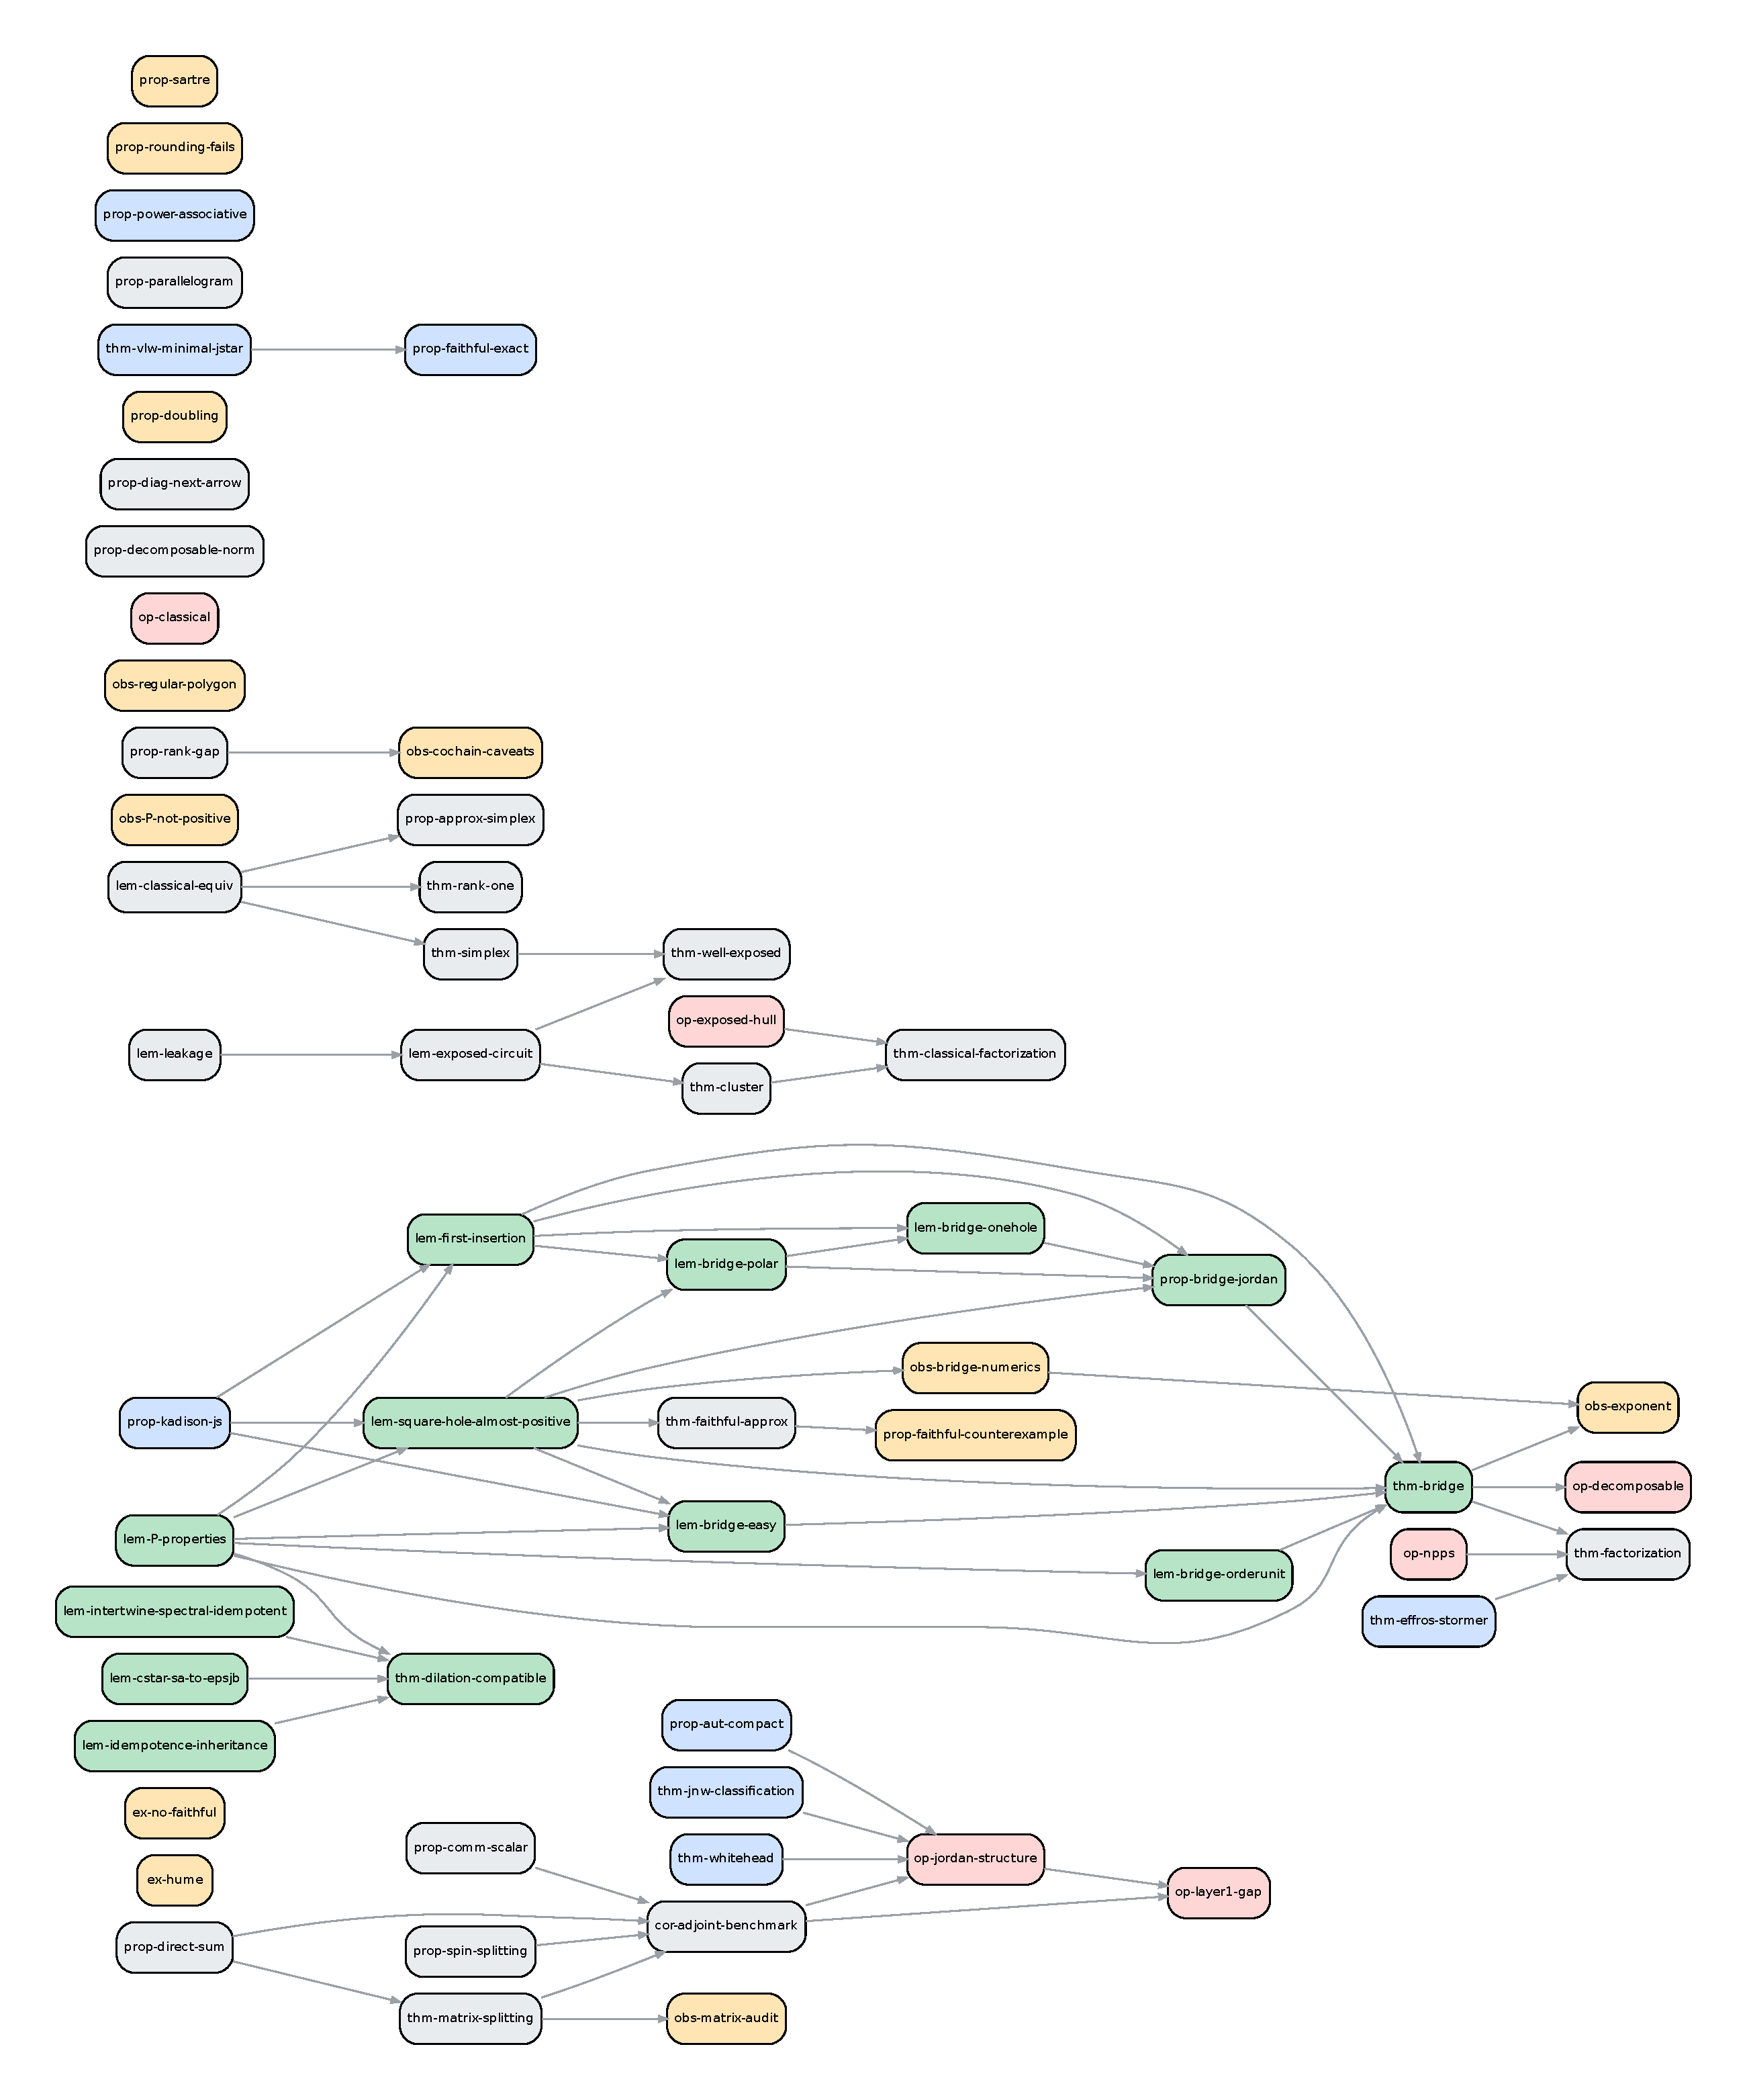
\includegraphics[width=\linewidth,height=0.9\textheight,keepaspectratio]{figures/dag}
\caption{The argument dependency graph, generated from the registry
\texttt{argument/lemmas/} by \texttt{scripts/gen-dag-figure.py}: one node per
result, each edge a dependency. Node colour:
\textcolor{afgreen}{$\blacksquare$~green} = af-validated (machine-checked);
grey = proved in prose but not yet formalised;
blue = cited from the literature;
red = open problem; amber = obstruction / no-go. The PDF is vector graphics:
zoom in a reader to inspect individual node labels.}
\label{fig:dag}
\end{figure}

\subsection{Outlook}

The picture that emerges is uniform. Mere positivity supplies Kadison's
inequality and hence a Jordan, not associative, structure; it supplies one hole
of control, hence the exponent $\sqrt\eta$; and it withholds the dilation that
would supply the second hole, the genuine positivity of $P$, and the
cb-norm-driven dimension-free homotopy. Each open problem is exactly the cost of
one missing piece of complete positivity: the exponent (\Cref{op:decomposable})
is the missing second hole; exact factorization (\Cref{op:npps}) is the missing
positivity of $P$; the abstract structure constant (\Cref{op:layer1-gap}) is
the missing cb-norm/order-unit homotopy, now sharpened by the exact-adjoint
benchmark but still requiring several pre-cohomological and approximate-module
components. None of the three is known to fail. Each has been reduced to
sharply stated remaining packages, not to an unconditional theorem.


\bibliographystyle{plain}
\bibliography{references}

\end{document}
